\documentclass[a4paper,14pt,oneside,openany]{memoir}

%%%%%%%%%%%%%%%%%%%%%%%%%%%%%%%%%%%%%%%%%%%%%%%%%%%%%%%%%%%%%%%%%%%%%%%%%%%%%%%%
%%%% Файл упрощённых настроек шаблона, общих для диссертации и автореферата %%%%
%%%%%%%%%%%%%%%%%%%%%%%%%%%%%%%%%%%%%%%%%%%%%%%%%%%%%%%%%%%%%%%%%%%%%%%%%%%%%%%%

%%% Режим черновика %%%
\makeatletter
\@ifundefined{c@draft}{
  \newcounter{draft}
  \setcounter{draft}{0}  % 0 --- чистовик (максимальное соблюдение ГОСТ)
                         % 1 --- черновик (отклонения от ГОСТ, но быстрая
                         %       сборка итоговых PDF)
}{}
\makeatother

%%% Пометки в тексте %%%
\makeatletter
\@ifundefined{c@showmarkup}{
  \newcounter{showmarkup}
  \setcounter{showmarkup}{1}  % 0 --- скрыть пометки
                              % 1 --- показывать пометки
}{}
\makeatother

%%% Использование в pdflatex шрифтов не по-умолчанию %%%
\makeatletter
\@ifundefined{c@usealtfont}{
  \newcounter{usealtfont}
  \setcounter{usealtfont}{1}    % 0 --- шрифты на базе Computer Modern
                                % 1 --- использовать пакет pscyr, при его
                                %       наличии
                                % 2 --- использовать пакет XCharter, при наличии
                                %       подходящей версии
}{}
\makeatother

%%% Использование в xelatex и lualatex семейств шрифтов %%%
\makeatletter
\@ifundefined{c@fontfamily}{
  \newcounter{fontfamily}
  \setcounter{fontfamily}{1}  % 0 --- CMU семейство. Используется как fallback;
                              % 1 --- Шрифты от MS (Times New Roman и компания)
                              % 2 --- Семейство Liberation
}{}
\makeatother


%%% Вывод типов ссылок в библиографии %%%
\makeatletter
\@ifundefined{c@mediadisplay}{
  \newcounter{mediadisplay}
  \setcounter{mediadisplay}{1}   % 0 --- не делать ничего; надписи [Текст] и
                                 %       [Эл. ресурс] будут выводиться только в ссылках с
                                 %       заполненным полем `media`;
                                 % 1 --- автоматически добавлять надпись [Текст] к ссылкам с
                                 %       незаполненным полем `media`; таким образом, у всех
                                 %       источников будет указан тип, что соответствует
                                 %       требованиям ГОСТ
                                 % 2 --- автоматически удалять надписи [Текст], [Эл. Ресурс] и др.;
                                 %       не соответствует ГОСТ
                                 % 3 --- автоматически удалять надпись [Текст];
                                 %       не соответствует ГОСТ
                                 % 4 --- автоматически удалять надпись [Эл. Ресурс];
                                 %       не соответствует ГОСТ
}{}
\makeatother

%%% Предкомпиляция tikz рисунков для ускорения работы %%%
\makeatletter
\@ifundefined{c@imgprecompile}{
  \newcounter{imgprecompile}
  \setcounter{imgprecompile}{0}   % 0 --- без предкомпиляции;
                                  % 1 --- пользоваться предварительно
                                  %       скомпилированными pdf вместо генерации
                                  %       заново из tikz
}{}
\makeatother
            % общие настройки шаблона
%%% Проверка используемого TeX-движка %%%
\newif\ifxetexorluatex   % определяем новый условный оператор (http://tex.stackexchange.com/a/47579)
\ifxetex
    \xetexorluatextrue
\else
    \ifluatex
        \xetexorluatextrue
    \else
        \xetexorluatexfalse
    \fi
\fi

\usepackage{etoolbox}[2015/08/02]   % Для продвинутой проверки разных условий
\providebool{presentation}

\usepackage{comment}    % Позволяет убирать блоки текста (добавляет
                        % окружение comment и команду \excludecomment)

%%% Поля и разметка страницы %%%
\usepackage{pdflscape}  % Для включения альбомных страниц
\usepackage{geometry}   % Для последующего задания полей

%%% Химические пакеты пакеты %%%
\usepackage{chemfig}

\usepackage{circuitikz}

%%% Математические пакеты %%%
\usepackage{amsthm,amsmath,amscd}   % Математические дополнения от AMS
\usepackage{amsfonts,amssymb}       % Математические дополнения от AMS
\usepackage{mathtools}              % Добавляет окружение multlined
\usepackage{xfrac}                  % Красивые дроби
\usepackage[
    locale = DE,
    list-separator       = {;\,},
    list-final-separator = {;\,},
    list-pair-separator  = {;\,},
    list-units           = single,
    range-units          = single,
    range-phrase={\text{\ensuremath{-}}},
    % quotient-mode        = fraction, % красивые дроби могут не соответствовать ГОСТ
    fraction-function    = \sfrac,
    separate-uncertainty,
    ]{siunitx}[=v2]                 % Размерности SI
\sisetup{inter-unit-product = \ensuremath{{}\cdot{}}}

% Кириллица в нумерации subequations
% Для правильной работы требуется выполнение сразу после загрузки пакетов
\patchcmd{\subequations}{\def\theequation{\theparentequation\alph{equation}}}
{\def\theequation{\theparentequation\asbuk{equation}}}
{\typeout{subequations patched}}{\typeout{subequations not patched}}

%%%% Установки для размера шрифта 14 pt %%%%
%% Формирование переменных и констант для сравнения (один раз для всех подключаемых файлов)%%
%% должно располагаться до вызова пакета fontspec или polyglossia, потому что они сбивают его работу
\newlength{\curtextsize}
\newlength{\bigtextsize}
\setlength{\bigtextsize}{13.9pt}

\makeatletter
%\show\f@size    % неплохо для отслеживания, но вызывает стопорение процесса,
                 % если документ компилируется без команды  -interaction=nonstopmode
\setlength{\curtextsize}{\f@size pt}
\makeatother

%%% Кодировки и шрифты %%%
\ifxetexorluatex
    \ifpresentation
        \providecommand*\autodot{} % quick fix for polyglossia 1.50
    \fi
    \PassOptionsToPackage{no-math}{fontspec}    % https://tex.stackexchange.com/a/26295/104425
    \usepackage{polyglossia}[2014/05/21]        % Поддержка многоязычности
                                        % (fontspec подгружается автоматически)
\else
   %%% Решение проблемы копирования текста в буфер кракозябрами
    \ifnumequal{\value{usealtfont}}{0}{}{
        \input glyphtounicode.tex
        \input glyphtounicode-cmr.tex %from pdfx package
        \pdfgentounicode=1
    }
    \usepackage{cmap}   % Улучшенный поиск русских слов в полученном pdf-файле
    \ifnumequal{\value{usealtfont}}{2}{}{
        \defaulthyphenchar=127  % Если стоит до fontenc, то переносы
                                % не впишутся в выделяемый текст при
                                % копировании его в буфер обмена
    }
    \usepackage{textcomp}
    \usepackage[T1,T2A]{fontenc}                    % Поддержка русских букв
    \ifnumequal{\value{usealtfont}}{1}{% Используется pscyr, при наличии
        \IfFileExists{pscyr.sty}{\usepackage{pscyr}}{}  % Подключение pscyr
    }{}
    \usepackage[utf8]{inputenc}[2014/04/30]         % Кодировка utf8
    \usepackage[english, russian]{babel}[2014/03/24]% Языки: русский, английский
    \makeatletter\AtBeginDocument{\let\@elt\relax}\makeatother % babel 3.40 fix
    \ifnumequal{\value{usealtfont}}{2}{
        % http://dxdy.ru/post1238763.html#p1238763
        \usepackage[scaled=0.914]{XCharter}[2017/12/19] % Подключение русифицированных шрифтов XCharter
        \usepackage[charter, vvarbb, scaled=1.048]{newtxmath}[2017/12/14]
        \ifpresentation
        \else
            \setDisplayskipStretch{-0.078}
        \fi
    }{}
\fi

%%% Оформление абзацев %%%
\ifpresentation
\else
    \indentafterchapter     % Красная строка после заголовков типа chapter
    \usepackage{indentfirst}
\fi

%%% Цвета %%%
\ifpresentation
\else
    \usepackage[dvipsnames, table, hyperref]{xcolor} % Совместимо с tikz
\fi

%%% Таблицы %%%
\usepackage{longtable,ltcaption} % Длинные таблицы
\usepackage{multirow,makecell}   % Улучшенное форматирование таблиц
\usepackage{tabu, tabulary}      % таблицы с автоматически подбирающейся
                                 % шириной столбцов (tabu обязательно
                                 % до hyperref вызывать)
\makeatletter
%https://github.com/tabu-issues-for-future-maintainer/tabu/issues/26
\@ifpackagelater{longtable}{2020/02/07}{
\def\tabuendlongtrial{%
    \LT@echunk  \global\setbox\LT@gbox \hbox{\unhbox\LT@gbox}\kern\wd\LT@gbox
                \LT@get@widths
}%
}{}
\makeatother

\usepackage{threeparttable}      % автоматический подгон ширины подписи таблицы

%%% Общее форматирование
\usepackage{soulutf8}% Поддержка переносоустойчивых подчёркиваний и зачёркиваний
\usepackage{icomma}  % Запятая в десятичных дробях

%%% Оптимизация расстановки переносов и длины последней строки абзаца
\IfFileExists{impnattypo.sty}{% проверка установленности пакета impnattypo
    \ifluatex
        \ifnumequal{\value{draft}}{1}{% Черновик
            \usepackage[hyphenation, lastparline, nosingleletter, homeoarchy,
            rivers, draft]{impnattypo}
        }{% Чистовик
            \usepackage[hyphenation, lastparline, nosingleletter]{impnattypo}
        }
    \else
        \usepackage[hyphenation, lastparline]{impnattypo}
    \fi
}{}

%% Векторная графика

\usepackage{tikz}                   % Продвинутый пакет векторной графики
\usetikzlibrary{chains}             % Для примера tikz рисунка
\usetikzlibrary{shapes.geometric}   % Для примера tikz рисунка
\usetikzlibrary{shapes.symbols}     % Для примера tikz рисунка
\usetikzlibrary{arrows}             % Для примера tikz рисунка

%%% Гиперссылки %%%
\ifxetexorluatex
    \let\CYRDZE\relax
\fi
\usepackage{hyperref}[2012/11/06]

%%% Изображения %%%
\usepackage{graphicx}[2014/04/25]   % Подключаем пакет работы с графикой
\usepackage{caption}                % Подписи рисунков и таблиц
\usepackage{subcaption}             % Подписи подрисунков и подтаблиц
\usepackage{pdfpages}               % Добавление внешних pdf файлов

%%% Счётчики %%%
\usepackage{aliascnt}
\usepackage[figure,table]{totalcount}   % Счётчик рисунков и таблиц
\usepackage{totcount}   % Пакет создания счётчиков на основе последнего номера
                        % подсчитываемого элемента (может требовать дважды
                        % компилировать документ)
\usepackage{totpages}   % Счётчик страниц, совместимый с hyperref (ссылается
                        % на номер последней страницы). Желательно ставить
                        % последним пакетом в преамбуле

%%% Продвинутое управление групповыми ссылками (пока только формулами) %%%
\ifpresentation
\else
    \usepackage[russian]{cleveref} % cleveref имеет сложности со считыванием
    % языка из babel. Такое решение русификации вывода выбрано вместо
    % определения в documentclass из опасности что-то лишнее передать во все
    % остальные пакеты, включая библиографию.

    % Добавление возможности использования пробелов в \labelcref
    % https://tex.stackexchange.com/a/340502/104425
    \usepackage{kvsetkeys}
    \makeatletter
    \let\org@@cref\@cref
    \renewcommand*{\@cref}[2]{%
        \edef\process@me{%
            \noexpand\org@@cref{#1}{\zap@space#2 \@empty}%
        }\process@me
    }
    \makeatother
\fi

\usepackage{placeins} % для \FloatBarrier

\ifnumequal{\value{draft}}{1}{% Черновик
    \usepackage[firstpage]{draftwatermark}
    \SetWatermarkText{DRAFT}
    \SetWatermarkFontSize{14pt}
    \SetWatermarkScale{15}
    \SetWatermarkAngle{45}
}{}

%%% Цитата, не приводимая в автореферате:
% возможно, актуальна только для biblatex
%\newcommand{\citeinsynopsis}[1]{\ifsynopsis\else ~\cite{#1} \fi}

% если текущий процесс запущен библиотекой tikz-external, то прекомпиляция должна быть включена
\ifdefined\tikzexternalrealjob
    \setcounter{imgprecompile}{1}
\fi

\ifnumequal{\value{imgprecompile}}{1}{% Только если у нас включена предкомпиляция
    \usetikzlibrary{external}   % подключение возможности предкомпиляции
    \tikzexternalize[prefix=images/cache/,optimize command away=\includepdf] % activate! % здесь можно указать отдельную папку для скомпилированных файлов
    \ifxetex
        \tikzset{external/up to date check={diff}}
    \fi
}{}




%%% Прикладные пакеты %%%
%\usepackage{calc}               % Пакет для расчётов параметров, например длины

%%% Для добавления Стр. над номерами страниц в оглавлении
%%% http://tex.stackexchange.com/a/306950
\usepackage{afterpage}

%%% Списки %%%
\usepackage{enumitem}

%%% Оформление списка обозначений
\usepackage[intoc]{nomencl}
\makenomenclature
\setlength{\nomitemsep}{-.8\parsep}





\usepackage{fr-longtable}    %ради \endlasthead

% Листинги с исходным кодом программ
\usepackage{fancyvrb}
\usepackage{listings}
\lccode`\~=0\relax %Без этого хака из-за особенностей пакета listings перестают работать конструкции с \MakeLowercase и т. п. в (xe|lua)latex

% Русская традиция начертания греческих букв
\usepackage{upgreek} % прямые греческие ради русской традиции

%%% Микротипографика
%\ifnumequal{\value{draft}}{0}{% Только если у нас режим чистовика
	%    \usepackage[final, babel, shrink=45]{microtype}[2016/05/14] % улучшает представление букв и слов в строках, может помочь при наличии отдельно висящих слов
	%}{}

% Отметка о версии черновика на каждой странице
% Чтобы работало надо в своей локальной копии по инструкции
% https://www.ctan.org/pkg/gitinfo2 создать небходимые файлы в папке
% ./git/hooks
% If you’re familiar with tweaking git, you can probably work it out for
% yourself. If not, I suggest you follow these steps:
% 1. First, you need a git repository and working tree. For this example,
% let’s suppose that the root of the working tree is in ~/compsci
% 2. Copy the file post-xxx-sample.txt (which is in the same folder of
% your TEX distribution as this pdf) into the git hooks directory in your
% working copy. In our example case, you should end up with a file called
% ~/compsci/.git/hooks/post-checkout
% 3. If you’re using a unix-like system, don’t forget to make the file executable.
% Just how you do this is outside the scope of this manual, but one
% possible way is with commands such as this:
% chmod g+x post-checkout.
% 4. Test your setup with “git checkout master” (or another suitable branch
% name). This should generate copies of gitHeadInfo.gin in the directories
% you intended.
% 5. Now make two more copies of this file in the same directory (hooks),
% calling them post-commit and post-merge, and you’re done. As before,
% users of unix-like systems should ensure these files are marked as
% executable.
\ifnumequal{\value{draft}}{1}{% Черновик
	\IfFileExists{.git/gitHeadInfo.gin}{
		\usepackage[mark,pcount]{gitinfo2}
		\renewcommand{\gitMark}{rev.\gitAbbrevHash\quad\gitCommitterEmail\quad\gitAuthorIsoDate}
		\renewcommand{\gitMarkFormat}{\rmfamily\color{Gray}\small\bfseries}
	}{}
}{}         % пакеты, которые нужны для шаблона

%%%%%%%%%%%%%%%%%%%%%%%%%%%%%%%%%%%%%%%%%%%%%%%%%%%%%%
%%%% Файл упрощённых настроек шаблона диссертации %%%%
%%%%%%%%%%%%%%%%%%%%%%%%%%%%%%%%%%%%%%%%%%%%%%%%%%%%%%

%%% Инициализирование переменных, не трогать!  %%%
\newcounter{intvl}
\newcounter{otstup}
\newcounter{contnumeq}
\newcounter{contnumfig}
\newcounter{contnumtab}
\newcounter{pgnum}
\newcounter{chapstyle}
\newcounter{headingdelim}
\newcounter{headingalign}
\newcounter{headingsize}
%%%%%%%%%%%%%%%%%%%%%%%%%%%%%%%%%%%%%%%%%%%%%%%%%%%%%%

%%% Область упрощённого управления оформлением %%%

%% Интервал между заголовками и между заголовком и текстом %%
% Заголовки отделяют от текста сверху и снизу
% тремя интервалами (ГОСТ Р 7.0.11-2011, 5.3.5)
\setcounter{intvl}{3}               % Коэффициент кратности к размеру шрифта

%% Отступы у заголовков в тексте %%
\setcounter{otstup}{0}              % 0 --- без отступа; 1 --- абзацный отступ

%% Нумерация формул, таблиц и рисунков %%
% Нумерация формул
\setcounter{contnumeq}{0}   % 0 --- пораздельно (во введении подряд,
                            %       без номера раздела);
                            % 1 --- сквозная нумерация по всей диссертации
% Нумерация рисунков
\setcounter{contnumfig}{0}  % 0 --- пораздельно (во введении подряд,
                            %       без номера раздела);
                            % 1 --- сквозная нумерация по всей диссертации
% Нумерация таблиц
\setcounter{contnumtab}{1}  % 0 --- пораздельно (во введении подряд,
                            %       без номера раздела);
                            % 1 --- сквозная нумерация по всей диссертации

%% Оглавление %%
\setcounter{pgnum}{1}       % 0 --- номера страниц никак не обозначены;
                            % 1 --- Стр. над номерами страниц (дважды
                            %       компилировать после изменения настройки)
\settocdepth{subsection}    % до какого уровня подразделов выносить в оглавление
\setsecnumdepth{subsection} % до какого уровня нумеровать подразделы


%% Текст и форматирование заголовков %%
\setcounter{chapstyle}{1}     % 0 --- разделы только под номером;
                              % 1 --- разделы с названием "Глава" перед номером
\setcounter{headingdelim}{1}  % 0 --- номер отделен пропуском в 1em или \quad;
                              % 1 --- номера разделов и приложений отделены
                              %       точкой с пробелом, подразделы пропуском
                              %       без точки;
                              % 2 --- номера разделов, подразделов и приложений
                              %       отделены точкой с пробелом.

%% Выравнивание заголовков в тексте %%
\setcounter{headingalign}{0}  % 0 --- по центру;
                              % 1 --- по левому краю

%% Размеры заголовков в тексте %%
\setcounter{headingsize}{0}   % 0 --- по ГОСТ, все всегда 14 пт;
                              % 1 --- пропорционально изменяющийся размер
                              %       в зависимости от базового шрифта

%% Подпись таблиц %%

% Смещение строк подписи после первой строки
\newcommand{\tabindent}{0cm}

% Тип форматирования заголовка таблицы:
% plain --- название и текст в одной строке
% split --- название и текст в разных строках
\newcommand{\tabformat}{plain}

%%% Настройки форматирования таблицы `plain`

% Выравнивание по центру подписи, состоящей из одной строки:
% true  --- выравнивать
% false --- не выравнивать
\newcommand{\tabsinglecenter}{false}

% Выравнивание подписи таблиц:
% justified   --- выравнивать как обычный текст («по ширине»)
% centering   --- выравнивать по центру
% centerlast  --- выравнивать по центру только последнюю строку
% centerfirst --- выравнивать по центру только первую строку (не рекомендуется)
% raggedleft  --- выравнивать по правому краю
% raggedright --- выравнивать по левому краю
\newcommand{\tabjust}{justified}

% Разделитель записи «Таблица #» и названия таблицы
\newcommand{\tablabelsep}{~\cyrdash\ }

%%% Настройки форматирования таблицы `split`

% Положение названия таблицы:
% \centering   --- выравнивать по центру
% \raggedleft  --- выравнивать по правому краю
% \raggedright --- выравнивать по левому краю
\newcommand{\splitformatlabel}{\raggedleft}

% Положение текста подписи:
% \centering   --- выравнивать по центру
% \raggedleft  --- выравнивать по правому краю
% \raggedright --- выравнивать по левому краю
\newcommand{\splitformattext}{\raggedright}

%% Подпись рисунков %%
%Разделитель записи «Рисунок #» и названия рисунка
\newcommand{\figlabelsep}{~\cyrdash\ }  % (ГОСТ 2.105, 4.3.1)
                                        % "--- здесь не работает

%%% Цвета гиперссылок %%%
% Latex color definitions: http://latexcolor.com/
\definecolor{linkcolor}{rgb}{0.9,0,0}
\definecolor{citecolor}{rgb}{0,0.6,0}
\definecolor{urlcolor}{rgb}{0,0,1}
%\definecolor{linkcolor}{rgb}{0,0,0} %black
%\definecolor{citecolor}{rgb}{0,0,0} %black
%\definecolor{urlcolor}{rgb}{0,0,0} %black
      % Упрощённые настройки шаблона
\newcommand{\statementOneRU}{
    Ваше первое положение на русском.
}
\newcommand{\statementOneEN}{
    Your first statement in English.
}


\newcommand{\statementTwoRU}{
    Ваше второе положение на русском.
}
\newcommand{\statementTwoEN}{
    Your second statement in English.
} % тут ваши положения 

%%% Кодировки и шрифты %%%
\ifxetexorluatex
    % Язык по-умолчанию русский с поддержкой приятных команд пакета babel
    \setmainlanguage[babelshorthands=true]{russian}
    % Дополнительный язык = английский (в американской вариации по-умолчанию)
    \setotherlanguage{english}

    % Проверка существования шрифтов. Недоступна в pdflatex
    \ifnumequal{\value{fontfamily}}{1}{
        \IfFontExistsTF{Times New Roman}{}{\setcounter{fontfamily}{0}}
    }{}
    \ifnumequal{\value{fontfamily}}{2}{
        \IfFontExistsTF{LiberationSerif}{}{\setcounter{fontfamily}{0}}
    }{}

    \ifnumequal{\value{fontfamily}}{0}{                    % Семейство шрифтов CMU. Используется как fallback
        \setmonofont{CMU Typewriter Text}                  % моноширинный шрифт
        \newfontfamily\cyrillicfonttt{CMU Typewriter Text} % моноширинный шрифт для кириллицы
        \defaultfontfeatures{Ligatures=TeX}                % стандартные лигатуры TeX, замены нескольких дефисов на тире и т. п. Настройки моноширинного шрифта должны идти до этой строки, чтобы при врезках кода программ в коде не применялись лигатуры и замены дефисов
        \setmainfont{CMU Serif}                            % Шрифт с засечками
        \newfontfamily\cyrillicfont{CMU Serif}             % Шрифт с засечками для кириллицы
        \setsansfont{CMU Sans Serif}                       % Шрифт без засечек
        \newfontfamily\cyrillicfontsf{CMU Sans Serif}      % Шрифт без засечек для кириллицы
    }

    \ifnumequal{\value{fontfamily}}{1}{                    % Семейство MS шрифтов
        \setmonofont{Courier New}                          % моноширинный шрифт
        \newfontfamily\cyrillicfonttt{Courier New}         % моноширинный шрифт для кириллицы
        \defaultfontfeatures{Ligatures=TeX}                % стандартные лигатуры TeX, замены нескольких дефисов на тире и т. п. Настройки моноширинного шрифта должны идти до этой строки, чтобы при врезках кода программ в коде не применялись лигатуры и замены дефисов
        \setmainfont{Times New Roman}                      % Шрифт с засечками
        \newfontfamily\cyrillicfont{Times New Roman}       % Шрифт с засечками для кириллицы
        \setsansfont{Arial}                                % Шрифт без засечек
        \newfontfamily\cyrillicfontsf{Arial}               % Шрифт без засечек для кириллицы
    }

    \ifnumequal{\value{fontfamily}}{2}{                    % Семейство шрифтов Liberation (https://pagure.io/liberation-fonts)
        \setmonofont{LiberationMono}[Scale=0.87] % моноширинный шрифт
        \newfontfamily\cyrillicfonttt{LiberationMono}[     % моноширинный шрифт для кириллицы
            Scale=0.87]
        \defaultfontfeatures{Ligatures=TeX}                % стандартные лигатуры TeX, замены нескольких дефисов на тире и т. п. Настройки моноширинного шрифта должны идти до этой строки, чтобы при врезках кода программ в коде не применялись лигатуры и замены дефисов
        \setmainfont{LiberationSerif}                      % Шрифт с засечками
        \newfontfamily\cyrillicfont{LiberationSerif}       % Шрифт с засечками для кириллицы
        \setsansfont{LiberationSans}                       % Шрифт без засечек
        \newfontfamily\cyrillicfontsf{LiberationSans}      % Шрифт без засечек для кириллицы
    }

\else
    \ifnumequal{\value{usealtfont}}{1}{% Используется pscyr, при наличии
        \IfFileExists{pscyr.sty}{\renewcommand{\rmdefault}{ftm}}{}
    }{}
\fi
            % Определение шрифтов (частичное)
%%% Шаблон %%%
\DeclareRobustCommand{\fixme}{\textcolor{red}}  % решаем проблему превращения
                                % названия цвета в результате \MakeUppercase,
                                % http://tex.stackexchange.com/a/187930,
                                % \DeclareRobustCommand protects \fixme
                                % from expanding inside \MakeUppercase
\AtBeginDocument{%
    \setlength{\parindent}{2.5em}                   % Абзацный отступ. Должен быть одинаковым по всему тексту и равен пяти знакам (ГОСТ Р 7.0.11-2011, 5.3.7).
}

%%% Таблицы %%%
\DeclareCaptionLabelSeparator{tabsep}{\tablabelsep} % нумерация таблиц
\DeclareCaptionFormat{split}{\splitformatlabel#1\par\splitformattext#3}

\captionsetup[table]{
        format=\tabformat,                % формат подписи (plain|hang)
        font=normal,                      % нормальные размер, цвет, стиль шрифта
        skip=.0pt,                        % отбивка под подписью
        parskip=.0pt,                     % отбивка между параграфами подписи
        position=above,                   % положение подписи
        justification=\tabjust,           % центровка
        indent=\tabindent,                % смещение строк после первой
        labelsep=tabsep,                  % разделитель
        singlelinecheck=\tabsinglecenter, % не выравнивать по центру, если умещается в одну строку
}

%%% Рисунки %%%
\DeclareCaptionLabelSeparator{figsep}{\figlabelsep} % нумерация рисунков

\captionsetup[figure]{
        format=plain,                     % формат подписи (plain|hang)
        font=normal,                      % нормальные размер, цвет, стиль шрифта
        skip=.0pt,                        % отбивка под подписью
        parskip=.0pt,                     % отбивка между параграфами подписи
        position=below,                   % положение подписи
        singlelinecheck=true,             % выравнивание по центру, если умещается в одну строку
        justification=centerlast,         % центровка
        labelsep=figsep,                  % разделитель
}

%%% Подписи подрисунков %%%
\DeclareCaptionSubType{figure}
\renewcommand\thesubfigure{\asbuk{subfigure}} % нумерация подрисунков
\DeclareCaptionFont{norm}{\fontsize{14pt}{16pt}\selectfont}
\newcommand{\subfigureskip}{0.pt}

\captionsetup[subfloat]{
        labelfont=norm,                 % нормальный размер подписей подрисунков
        textfont=norm,                  % нормальный размер подписей подрисунков
        labelsep=space,                 % разделитель
        labelformat=brace,              % одна скобка справа от номера
        justification=centering,        % центровка
        singlelinecheck=true,           % выравнивание по центру, если умещается в одну строку
        skip=\subfigureskip,            % отбивка над подписью
        parskip=.0pt,                   % отбивка между параграфами подписи
        position=below,                 % положение подписи
}

%%% Настройки ссылок на рисунки, таблицы и др. %%%
% команды \cref...format отвечают за форматирование при помощи команды \cref
% команды \labelcref...format отвечают за форматирование при помощи команды \labelcref

\ifpresentation
\else
    \crefdefaultlabelformat{#2#1#3}

    % Уравнение
    \crefformat{equation}{(#2#1#3)} % одиночная ссылка с приставкой
    \labelcrefformat{equation}{(#2#1#3)} % одиночная ссылка без приставки
    \crefrangeformat{equation}{(#3#1#4) \cyrdash~(#5#2#6)} % диапазон ссылок с приставкой
    \labelcrefrangeformat{equation}{(#3#1#4) \cyrdash~(#5#2#6)} % диапазон ссылок без приставки
    \crefmultiformat{equation}{(#2#1#3)}{ и~(#2#1#3)}{, (#2#1#3)}{ и~(#2#1#3)} % перечисление ссылок с приставкой
    \labelcrefmultiformat{equation}{(#2#1#3)}{ и~(#2#1#3)}{, (#2#1#3)}{ и~(#2#1#3)} % перечисление без приставки

    % Подуравнение
    \crefformat{subequation}{(#2#1#3)} % одиночная ссылка с приставкой
    \labelcrefformat{subequation}{(#2#1#3)} % одиночная ссылка без приставки
    \crefrangeformat{subequation}{(#3#1#4) \cyrdash~(#5#2#6)} % диапазон ссылок с приставкой
    \labelcrefrangeformat{subequation}{(#3#1#4) \cyrdash~(#5#2#6)} % диапазон ссылок без приставки
    \crefmultiformat{subequation}{(#2#1#3)}{ и~(#2#1#3)}{, (#2#1#3)}{ и~(#2#1#3)} % перечисление ссылок с приставкой
    \labelcrefmultiformat{subequation}{(#2#1#3)}{ и~(#2#1#3)}{, (#2#1#3)}{ и~(#2#1#3)} % перечисление без приставки

    % Глава
    \crefformat{chapter}{#2#1#3} % одиночная ссылка с приставкой
    \labelcrefformat{chapter}{#2#1#3} % одиночная ссылка без приставки
    \crefrangeformat{chapter}{#3#1#4 \cyrdash~#5#2#6} % диапазон ссылок с приставкой
    \labelcrefrangeformat{chapter}{#3#1#4 \cyrdash~#5#2#6} % диапазон ссылок без приставки
    \crefmultiformat{chapter}{#2#1#3}{ и~#2#1#3}{, #2#1#3}{ и~#2#1#3} % перечисление ссылок с приставкой
    \labelcrefmultiformat{chapter}{#2#1#3}{ и~#2#1#3}{, #2#1#3}{ и~#2#1#3} % перечисление без приставки

    % Параграф
    \crefformat{section}{#2#1#3} % одиночная ссылка с приставкой
    \labelcrefformat{section}{#2#1#3} % одиночная ссылка без приставки
    \crefrangeformat{section}{#3#1#4 \cyrdash~#5#2#6} % диапазон ссылок с приставкой
    \labelcrefrangeformat{section}{#3#1#4 \cyrdash~#5#2#6} % диапазон ссылок без приставки
    \crefmultiformat{section}{#2#1#3}{ и~#2#1#3}{, #2#1#3}{ и~#2#1#3} % перечисление ссылок с приставкой
    \labelcrefmultiformat{section}{#2#1#3}{ и~#2#1#3}{, #2#1#3}{ и~#2#1#3} % перечисление без приставки

    % Приложение
    \crefformat{appendix}{#2#1#3} % одиночная ссылка с приставкой
    \labelcrefformat{appendix}{#2#1#3} % одиночная ссылка без приставки
    \crefrangeformat{appendix}{#3#1#4 \cyrdash~#5#2#6} % диапазон ссылок с приставкой
    \labelcrefrangeformat{appendix}{#3#1#4 \cyrdash~#5#2#6} % диапазон ссылок без приставки
    \crefmultiformat{appendix}{#2#1#3}{ и~#2#1#3}{, #2#1#3}{ и~#2#1#3} % перечисление ссылок с приставкой
    \labelcrefmultiformat{appendix}{#2#1#3}{ и~#2#1#3}{, #2#1#3}{ и~#2#1#3} % перечисление без приставки

    % Рисунок
    \crefformat{figure}{#2#1#3} % одиночная ссылка с приставкой
    \labelcrefformat{figure}{#2#1#3} % одиночная ссылка без приставки
    \crefrangeformat{figure}{#3#1#4 \cyrdash~#5#2#6} % диапазон ссылок с приставкой
    \labelcrefrangeformat{figure}{#3#1#4 \cyrdash~#5#2#6} % диапазон ссылок без приставки
    \crefmultiformat{figure}{#2#1#3}{ и~#2#1#3}{, #2#1#3}{ и~#2#1#3} % перечисление ссылок с приставкой
    \labelcrefmultiformat{figure}{#2#1#3}{ и~#2#1#3}{, #2#1#3}{ и~#2#1#3} % перечисление без приставки

    % Таблица
    \crefformat{table}{#2#1#3} % одиночная ссылка с приставкой
    \labelcrefformat{table}{#2#1#3} % одиночная ссылка без приставки
    \crefrangeformat{table}{#3#1#4 \cyrdash~#5#2#6} % диапазон ссылок с приставкой
    \labelcrefrangeformat{table}{#3#1#4 \cyrdash~#5#2#6} % диапазон ссылок без приставки
    \crefmultiformat{table}{#2#1#3}{ и~#2#1#3}{, #2#1#3}{ и~#2#1#3} % перечисление ссылок с приставкой
    \labelcrefmultiformat{table}{#2#1#3}{ и~#2#1#3}{, #2#1#3}{ и~#2#1#3} % перечисление без приставки

    % Листинг
    \crefformat{lstlisting}{#2#1#3} % одиночная ссылка с приставкой
    \labelcrefformat{lstlisting}{#2#1#3} % одиночная ссылка без приставки
    \crefrangeformat{lstlisting}{#3#1#4 \cyrdash~#5#2#6} % диапазон ссылок с приставкой
    \labelcrefrangeformat{lstlisting}{#3#1#4 \cyrdash~#5#2#6} % диапазон ссылок без приставки
    \crefmultiformat{lstlisting}{#2#1#3}{ и~#2#1#3}{, #2#1#3}{ и~#2#1#3} % перечисление ссылок с приставкой
    \labelcrefmultiformat{lstlisting}{#2#1#3}{ и~#2#1#3}{, #2#1#3}{ и~#2#1#3} % перечисление без приставки

    % Листинг
    \crefformat{ListingEnv}{#2#1#3} % одиночная ссылка с приставкой
    \labelcrefformat{ListingEnv}{#2#1#3} % одиночная ссылка без приставки
    \crefrangeformat{ListingEnv}{#3#1#4 \cyrdash~#5#2#6} % диапазон ссылок с приставкой
    \labelcrefrangeformat{ListingEnv}{#3#1#4 \cyrdash~#5#2#6} % диапазон ссылок без приставки
    \crefmultiformat{ListingEnv}{#2#1#3}{ и~#2#1#3}{, #2#1#3}{ и~#2#1#3} % перечисление ссылок с приставкой
    \labelcrefmultiformat{ListingEnv}{#2#1#3}{ и~#2#1#3}{, #2#1#3}{ и~#2#1#3} % перечисление без приставки
\fi

%%% Настройки гиперссылок %%%
\ifluatex
    \hypersetup{
        unicode,                % Unicode encoded PDF strings
    }
\fi

\hypersetup{
    linktocpage=true,           % ссылки с номера страницы в оглавлении, списке таблиц и списке рисунков
%    linktoc=all,                % both the section and page part are links
%    pdfpagelabels=false,        % set PDF page labels (true|false)
    plainpages=false,           % Forces page anchors to be named by the Arabic form  of the page number, rather than the formatted form
    colorlinks,                 % ссылки отображаются раскрашенным текстом, а не раскрашенным прямоугольником, вокруг текста
    linkcolor={linkcolor},      % цвет ссылок типа ref, eqref и подобных
    citecolor={citecolor},      % цвет ссылок-цитат
    urlcolor={urlcolor},        % цвет гиперссылок
%    hidelinks,                  % Hide links (removing color and border)
    pdftitle={PhD Thesis},    % Заголовок
    pdfauthor={Author},  % Автор
    pdfsubject={01.04.05 Optics},      % Тема
%    pdfcreator={Создатель},     % Создатель, Приложение
%    pdfproducer={Производитель},% Производитель, Производитель PDF
    pdfkeywords={physics},    % Ключевые слова
    pdflang={ru},
}
\ifnumequal{\value{draft}}{1}{% Черновик
    \hypersetup{
        draft,
    }
}{}

%%% Списки %%%
% Используем короткое тире (endash) для ненумерованных списков (ГОСТ 2.105-95, пункт 4.1.7, требует дефиса, но так лучше смотрится)
\renewcommand{\labelitemi}{\normalfont\bfseries{--}}

% Перечисление строчными буквами латинского алфавита (ГОСТ 2.105-95, 4.1.7)
%\renewcommand{\theenumi}{\alph{enumi}}
%\renewcommand{\labelenumi}{\theenumi)}

% Перечисление строчными буквами русского алфавита (ГОСТ 2.105-95, 4.1.7)
\makeatletter
\AddEnumerateCounter{\asbuk}{\russian@alph}{щ}      % Управляем списками/перечислениями через пакет enumitem, а он 'не знает' про asbuk, потому 'учим' его
\makeatother
%\renewcommand{\theenumi}{\asbuk{enumi}} %первый уровень нумерации
%\renewcommand{\labelenumi}{\theenumi)} %первый уровень нумерации
\renewcommand{\theenumii}{\asbuk{enumii}} %второй уровень нумерации
\renewcommand{\labelenumii}{\theenumii)} %второй уровень нумерации
\renewcommand{\theenumiii}{\arabic{enumiii}} %третий уровень нумерации
\renewcommand{\labelenumiii}{\theenumiii)} %третий уровень нумерации

\setlist{nosep,%                                    % Единый стиль для всех списков (пакет enumitem), без дополнительных интервалов.
    labelindent=\parindent,leftmargin=*%            % Каждый пункт, подпункт и перечисление записывают с абзацного отступа (ГОСТ 2.105-95, 4.1.8)
}

%%% Правильная нумерация приложений, рисунков и формул %%%
%% По ГОСТ 2.105, п. 4.3.8 Приложения обозначают заглавными буквами русского алфавита,
%% начиная с А, за исключением букв Ё, З, Й, О, Ч, Ь, Ы, Ъ.
%% Здесь также переделаны все нумерации русскими буквами.
\ifxetexorluatex
    \makeatletter
    \def\russian@Alph#1{\ifcase#1\or
       А\or Б\or В\or Г\or Д\or Е\or Ж\or
       И\or К\or Л\or М\or Н\or
       П\or Р\or С\or Т\or У\or Ф\or Х\or
       Ц\or Ш\or Щ\or Э\or Ю\or Я\else\xpg@ill@value{#1}{russian@Alph}\fi}
    \def\russian@alph#1{\ifcase#1\or
       а\or б\or в\or г\or д\or е\or ж\or
       и\or к\or л\or м\or н\or
       п\or р\or с\or т\or у\or ф\or х\or
       ц\or ш\or щ\or э\or ю\or я\else\xpg@ill@value{#1}{russian@alph}\fi}
    \def\cyr@Alph#1{\ifcase#1\or
        А\or Б\or В\or Г\or Д\or Е\or Ж\or
        И\or К\or Л\or М\or Н\or
        П\or Р\or С\or Т\or У\or Ф\or Х\or
        Ц\or Ш\or Щ\or Э\or Ю\or Я\else\xpg@ill@value{#1}{cyr@Alph}\fi}
    \def\cyr@alph#1{\ifcase#1\or
        а\or б\or в\or г\or д\or е\or ж\or
        и\or к\or л\or м\or н\or
        п\or р\or с\or т\or у\or ф\or х\or
        ц\or ш\or щ\or э\or ю\or я\else\xpg@ill@value{#1}{cyr@alph}\fi}
    \makeatother
\else
    \makeatletter
    \if@uni@ode
      \def\russian@Alph#1{\ifcase#1\or
        А\or Б\or В\or Г\or Д\or Е\or Ж\or
        И\or К\or Л\or М\or Н\or
        П\or Р\or С\or Т\or У\or Ф\or Х\or
        Ц\or Ш\or Щ\or Э\or Ю\or Я\else\@ctrerr\fi}
    \else
      \def\russian@Alph#1{\ifcase#1\or
        \CYRA\or\CYRB\or\CYRV\or\CYRG\or\CYRD\or\CYRE\or\CYRZH\or
        \CYRI\or\CYRK\or\CYRL\or\CYRM\or\CYRN\or
        \CYRP\or\CYRR\or\CYRS\or\CYRT\or\CYRU\or\CYRF\or\CYRH\or
        \CYRC\or\CYRSH\or\CYRSHCH\or\CYREREV\or\CYRYU\or
        \CYRYA\else\@ctrerr\fi}
    \fi
    \if@uni@ode
      \def\russian@alph#1{\ifcase#1\or
        а\or б\or в\or г\or д\or е\or ж\or
        и\or к\or л\or м\or н\or
        п\or р\or с\or т\or у\or ф\or х\or
        ц\or ш\or щ\or э\or ю\or я\else\@ctrerr\fi}
    \else
      \def\russian@alph#1{\ifcase#1\or
        \cyra\or\cyrb\or\cyrv\or\cyrg\or\cyrd\or\cyre\or\cyrzh\or
        \cyri\or\cyrk\or\cyrl\or\cyrm\or\cyrn\or
        \cyrp\or\cyrr\or\cyrs\or\cyrt\or\cyru\or\cyrf\or\cyrh\or
        \cyrc\or\cyrsh\or\cyrshch\or\cyrerev\or\cyryu\or
        \cyrya\else\@ctrerr\fi}
    \fi
    \makeatother
\fi


%%http://www.linux.org.ru/forum/general/6993203#comment-6994589 (используется totcount)
\makeatletter
\def\formtotal#1#2#3#4#5{%
    \newcount\@c
    \@c\totvalue{#1}\relax
    \newcount\@last
    \newcount\@pnul
    \@last\@c\relax
    \divide\@last 10
    \@pnul\@last\relax
    \divide\@pnul 10
    \multiply\@pnul-10
    \advance\@pnul\@last
    \multiply\@last-10
    \advance\@last\@c
    #2%
    \ifnum\@pnul=1#5\else%
    \ifcase\@last#5\or#3\or#4\or#4\or#4\else#5\fi
    \fi
}
\makeatother

\newcommand{\formbytotal}[5]{\total{#1}~\formtotal{#1}{#2}{#3}{#4}{#5}}

%%% Команды рецензирования %%%
\ifboolexpr{ (test {\ifnumequal{\value{draft}}{1}}) or (test {\ifnumequal{\value{showmarkup}}{1}})}{
        \newrobustcmd{\todo}[1]{\textcolor{red}{#1}}
        \newrobustcmd{\note}[2][]{\ifstrempty{#1}{#2}{\textcolor{#1}{#2}}}
        \newenvironment{commentbox}[1][]%
        {\ifstrempty{#1}{}{\color{#1}}}%
        {}
}{
        \newrobustcmd{\todo}[1]{}
        \newrobustcmd{\note}[2][]{}
        \excludecomment{commentbox}
}



%%% Переопределение именований, если иначе не сработает %%%
%\gappto\captionsrussian{
	%    \renewcommand{\chaptername}{Глава}
	%    \renewcommand{\appendixname}{Приложение} % (ГОСТ Р 7.0.11-2011, 5.7)
	%}

%%% Изображения %%%
\graphicspath{{images/}{Dissertation/images/}}         % Пути к изображениям

%%% Интервалы %%%
%% По ГОСТ Р 7.0.11-2011, пункту 5.3.6 требуется полуторный интервал
%% Реализация средствами класса (на основе setspace) ближе к типографской классике.
%% И правит сразу и в таблицах (если со звёздочкой)
%\DoubleSpacing*     % Двойной интервал
\OnehalfSpacing*    % Полуторный интервал
%\setSpacing{1.42}   % Полуторный интервал, подобный Ворду (возможно, стоит включать вместе с предыдущей строкой)

%%% Макет страницы %%%
% Выставляем значения полей (ГОСТ 7.0.11-2011, 5.3.7)
\geometry{a4paper, top=2cm, bottom=2cm, left=2.5cm, right=1cm, nofoot, nomarginpar} %, heightrounded, showframe
\setlength{\topskip}{0pt}   %размер дополнительного верхнего поля
\setlength{\footskip}{12.3pt} % снимет warning, согласно https://tex.stackexchange.com/a/334346

%%% Выравнивание и переносы %%%
%% http://tex.stackexchange.com/questions/241343/what-is-the-meaning-of-fussy-sloppy-emergencystretch-tolerance-hbadness
%% http://www.latex-community.org/forum/viewtopic.php?p=70342#p70342
\tolerance 1414
\hbadness 1414
\emergencystretch 1.5em % В случае проблем регулировать в первую очередь
\hfuzz 0.3pt
\vfuzz \hfuzz
%\raggedbottom
%\sloppy                 % Избавляемся от переполнений
\clubpenalty=10000      % Запрещаем разрыв страницы после первой строки абзаца
\widowpenalty=10000     % Запрещаем разрыв страницы после последней строки абзаца
\brokenpenalty=4991     % Ограничение на разрыв страницы, если строка заканчивается переносом

%%% Блок управления параметрами для выравнивания заголовков в тексте %%%
\newlength{\otstuplen}
\setlength{\otstuplen}{\theotstup\parindent}
\ifnumequal{\value{headingalign}}{0}{% выравнивание заголовков в тексте
	\newcommand{\hdngalign}{\centering}                % по центру
	\newcommand{\hdngaligni}{}% по центру
	\setlength{\otstuplen}{0pt}
}{%
	\newcommand{\hdngalign}{}                 % по левому краю
	\newcommand{\hdngaligni}{\hspace{\otstuplen}}      % по левому краю
} % В обоих случаях вроде бы без переноса, как и надо (ГОСТ Р 7.0.11-2011, 5.3.5)

%%% Оглавление %%%
\renewcommand{\cftchapterdotsep}{\cftdotsep}                % отбивка точками до номера страницы начала главы/раздела

%% Переносить слова в заголовке не допускается (ГОСТ Р 7.0.11-2011, 5.3.5). Заголовки в оглавлении должны точно повторять заголовки в тексте (ГОСТ Р 7.0.11-2011, 5.2.3). Прямого указания на запрет переносов в оглавлении нет, но по той же логике невнесения искажений в смысл, лучше в оглавлении не переносить:
\setrmarg{2.55em plus1fil}                             %To have the (sectional) titles in the ToC, etc., typeset ragged right with no hyphenation
\renewcommand{\cftchapterpagefont}{\normalfont}        % нежирные номера страниц у глав в оглавлении
\renewcommand{\cftchapterleader}{\cftdotfill{\cftchapterdotsep}}% нежирные точки до номеров страниц у глав в оглавлении
%\renewcommand{\cftchapterfont}{}                       % нежирные названия глав в оглавлении

\ifnumgreater{\value{headingdelim}}{0}{%
	\renewcommand\cftchapteraftersnum{.\space}       % добавляет точку с пробелом после номера раздела в оглавлении
}{}
\ifnumgreater{\value{headingdelim}}{1}{%
	\renewcommand\cftsectionaftersnum{.\space}       % добавляет точку с пробелом после номера подраздела в оглавлении
	\renewcommand\cftsubsectionaftersnum{.\space}    % добавляет точку с пробелом после номера подподраздела в оглавлении
	\renewcommand\cftsubsubsectionaftersnum{.\space} % добавляет точку с пробелом после номера подподподраздела в оглавлении
	\AfterEndPreamble{% без этого polyglossia сама всё переопределяет
		\setsecnumformat{\csname the#1\endcsname.\space}
	}
}{%
	\AfterEndPreamble{% без этого polyglossia сама всё переопределяет
		\setsecnumformat{\csname the#1\endcsname\quad}
	}
}

\renewcommand*{\cftappendixname}{\appendixname\space} % Слово Приложение в оглавлении

%%% Колонтитулы %%%
% Порядковый номер страницы печатают на середине верхнего поля страницы (ГОСТ Р 7.0.11-2011, 5.3.8)
\makeevenhead{plain}{}{\rmfamily\thepage}{}
\makeoddhead{plain}{}{\rmfamily\thepage}{}
\makeevenfoot{plain}{}{}{}
\makeoddfoot{plain}{}{}{}
\pagestyle{plain}

%%% добавить Стр. над номерами страниц в оглавлении
%%% http://tex.stackexchange.com/a/306950
\newif\ifendTOC

\newcommand*{\tocheader}{
	\ifnumequal{\value{pgnum}}{1}{%
		\ifendTOC\else\hbox to \linewidth%
		{\noindent{}~\hfill{Стр.}}\par%
		\ifnumless{\value{page}}{3}{}{%
			\vspace{0.5\onelineskip}
		}
		\afterpage{\tocheader}
		\fi%
	}{}%
}%

%%% Оформление заголовков глав, разделов, подразделов %%%
%% Работа должна быть выполнена ... размером шрифта 12-14 пунктов (ГОСТ Р 7.0.11-2011, 5.3.8). То есть не должно быть надписей шрифтом более 14. Так и поставим.
%% Эти установки будут давать одинаковый результат независимо от выбора базовым шрифтом 12 пт или 14 пт
\newcommand{\basegostsectionfont}{\fontsize{14pt}{16pt}\selectfont\bfseries}

\makechapterstyle{thesisgost}{%
	\chapterstyle{default}
	\setlength{\beforechapskip}{0pt}
	\setlength{\midchapskip}{0pt}
	\setlength{\afterchapskip}{\theintvl\curtextsize}
	\renewcommand*{\chapnamefont}{\basegostsectionfont}
	\renewcommand*{\chapnumfont}{\basegostsectionfont}
	\renewcommand*{\chaptitlefont}{\basegostsectionfont}
	\renewcommand*{\chapterheadstart}{}
	\ifnumgreater{\value{headingdelim}}{0}{%
		\renewcommand*{\afterchapternum}{.\space}   % добавляет точку с пробелом после номера раздела
	}{%
		\renewcommand*{\afterchapternum}{\quad}     % добавляет \quad после номера раздела
	}
	\renewcommand*{\printchapternum}{\hdngaligni\hdngalign\chapnumfont \thechapter}
	\renewcommand*{\printchaptername}{}
	\renewcommand*{\printchapternonum}{\hdngaligni\hdngalign}
}

\makeatletter
\makechapterstyle{thesisgostchapname}{%
	\chapterstyle{thesisgost}
	\renewcommand*{\printchapternum}{\chapnumfont \thechapter}
	\renewcommand*{\printchaptername}{\hdngaligni\hdngalign\chapnamefont \@chapapp} %
}
\makeatother

\chapterstyle{thesisgost}

\setsecheadstyle{\basegostsectionfont\hdngalign}
\setsecindent{\otstuplen}

\setsubsecheadstyle{\basegostsectionfont\hdngalign}
\setsubsecindent{\otstuplen}

\setsubsubsecheadstyle{\basegostsectionfont\hdngalign}
\setsubsubsecindent{\otstuplen}

\sethangfrom{\noindent #1} %все заголовки подразделов центрируются с учетом номера, как block

\ifnumequal{\value{chapstyle}}{1}{%
	\chapterstyle{thesisgostchapname}
	\renewcommand*{\cftchaptername}{\chaptername\space} % будет вписано слово Глава перед каждым номером раздела в оглавлении
}{}%

%%% Интервалы между заголовками
\setbeforesecskip{\theintvl\curtextsize}% Заголовки отделяют от текста сверху и снизу тремя интервалами (ГОСТ Р 7.0.11-2011, 5.3.5).
\setaftersecskip{\theintvl\curtextsize}
\setbeforesubsecskip{\theintvl\curtextsize}
\setaftersubsecskip{\theintvl\curtextsize}
\setbeforesubsubsecskip{\theintvl\curtextsize}
\setaftersubsubsecskip{\theintvl\curtextsize}

%%% Вертикальные интервалы глав (\chapter) в оглавлении как и у заголовков
% раскомментировать следующие 2
% \setlength{\cftbeforechapterskip}{0pt plus 0pt}   % ИЛИ эти 2 строки из учебника
% \renewcommand*{\insertchapterspace}{}
% или эту
% \renewcommand*{\cftbeforechapterskip}{0em}


%%% Блок дополнительного управления размерами заголовков
\ifnumequal{\value{headingsize}}{1}{% Пропорциональные заголовки и базовый шрифт 14 пт
	\renewcommand{\basegostsectionfont}{\large\bfseries}
	\renewcommand*{\chapnamefont}{\Large\bfseries}
	\renewcommand*{\chapnumfont}{\Large\bfseries}
	\renewcommand*{\chaptitlefont}{\Large\bfseries}
}{}

%%% Счётчики %%%

%% Упрощённые настройки шаблона диссертации: нумерация формул, таблиц, рисунков
\ifnumequal{\value{contnumeq}}{1}{%
	\counterwithout{equation}{chapter} % Убираем связанность номера формулы с номером главы/раздела
}{}
\ifnumequal{\value{contnumfig}}{1}{%
	\counterwithout{figure}{chapter}   % Убираем связанность номера рисунка с номером главы/раздела
}{}
\ifnumequal{\value{contnumtab}}{1}{%
	\counterwithout{table}{chapter}    % Убираем связанность номера таблицы с номером главы/раздела
}{}

\AfterEndPreamble{
	%% регистрируем счётчики в системе totcounter
	\regtotcounter{totalcount@figure}
	\regtotcounter{totalcount@table}       % Если иным способом поставить в преамбуле то ошибка в числе таблиц
	\regtotcounter{TotPages}               % Если иным способом поставить в преамбуле то ошибка в числе страниц
	\newtotcounter{totalappendix}
	\newtotcounter{totalchapter}
}


% для вертикального центрирования ячеек в tabulary
\def\zz{\ifx\[$\else\aftergroup\zzz\fi}
%$ \] % <-- чиним подсветку синтаксиса в некоторых редакторах
\def\zzz{\setbox0\lastbox
	\dimen0\dimexpr\extrarowheight + \ht0-\dp0\relax
	\setbox0\hbox{\raise-.5\dimen0\box0}%
	\ht0=\dimexpr\ht0+\extrarowheight\relax
	\dp0=\dimexpr\dp0+\extrarowheight\relax
	\box0
}

\lstdefinelanguage{Renhanced}%
{keywords={abbreviate,abline,abs,acos,acosh,action,add1,add,%
		aggregate,alias,Alias,alist,all,anova,any,aov,aperm,append,apply,%
		approx,approxfun,apropos,Arg,args,array,arrows,as,asin,asinh,%
		atan,atan2,atanh,attach,attr,attributes,autoload,autoloader,ave,%
		axis,backsolve,barplot,basename,besselI,besselJ,besselK,besselY,%
		beta,binomial,body,box,boxplot,break,browser,bug,builtins,bxp,by,%
		c,C,call,Call,case,cat,category,cbind,ceiling,character,char,%
		charmatch,check,chol,chol2inv,choose,chull,class,close,cm,codes,%
		coef,coefficients,co,col,colnames,colors,colours,commandArgs,%
		comment,complete,complex,conflicts,Conj,contents,contour,%
		contrasts,contr,control,helmert,contrib,convolve,cooks,coords,%
		distance,coplot,cor,cos,cosh,count,fields,cov,covratio,wt,CRAN,%
		create,crossprod,cummax,cummin,cumprod,cumsum,curve,cut,cycle,D,%
		data,dataentry,date,dbeta,dbinom,dcauchy,dchisq,de,debug,%
		debugger,Defunct,default,delay,delete,deltat,demo,de,density,%
		deparse,dependencies,Deprecated,deriv,description,detach,%
		dev2bitmap,dev,cur,deviance,off,prev,,dexp,df,dfbetas,dffits,%
		dgamma,dgeom,dget,dhyper,diag,diff,digamma,dim,dimnames,dir,%
		dirname,dlnorm,dlogis,dnbinom,dnchisq,dnorm,do,dotplot,double,%
		download,dpois,dput,drop,drop1,dsignrank,dt,dummy,dump,dunif,%
		duplicated,dweibull,dwilcox,dyn,edit,eff,effects,eigen,else,%
		emacs,end,environment,env,erase,eval,equal,evalq,example,exists,%
		exit,exp,expand,expression,External,extract,extractAIC,factor,%
		fail,family,fft,file,filled,find,fitted,fivenum,fix,floor,for,%
		For,formals,format,formatC,formula,Fortran,forwardsolve,frame,%
		frequency,ftable,ftable2table,function,gamma,Gamma,gammaCody,%
		gaussian,gc,gcinfo,gctorture,get,getenv,geterrmessage,getOption,%
		getwd,gl,glm,globalenv,gnome,GNOME,graphics,gray,grep,grey,grid,%
		gsub,hasTsp,hat,heat,help,hist,home,hsv,httpclient,I,identify,if,%
		ifelse,Im,image,\%in\%,index,influence,measures,inherits,install,%
		installed,integer,interaction,interactive,Internal,intersect,%
		inverse,invisible,IQR,is,jitter,kappa,kronecker,labels,lapply,%
		layout,lbeta,lchoose,lcm,legend,length,levels,lgamma,library,%
		licence,license,lines,list,lm,load,local,locator,log,log10,log1p,%
		log2,logical,loglin,lower,lowess,ls,lsfit,lsf,ls,machine,Machine,%
		mad,mahalanobis,make,link,margin,match,Math,matlines,mat,matplot,%
		matpoints,matrix,max,mean,median,memory,menu,merge,methods,min,%
		missing,Mod,mode,model,response,mosaicplot,mtext,mvfft,na,nan,%
		names,omit,nargs,nchar,ncol,NCOL,new,next,NextMethod,nextn,%
		nlevels,nlm,noquote,NotYetImplemented,NotYetUsed,nrow,NROW,null,%
		numeric,\%o\%,objects,offset,old,on,Ops,optim,optimise,optimize,%
		options,or,order,ordered,outer,package,packages,page,pairlist,%
		pairs,palette,panel,par,parent,parse,paste,path,pbeta,pbinom,%
		pcauchy,pchisq,pentagamma,persp,pexp,pf,pgamma,pgeom,phyper,pico,%
		pictex,piechart,Platform,plnorm,plogis,plot,pmatch,pmax,pmin,%
		pnbinom,pnchisq,pnorm,points,poisson,poly,polygon,polyroot,pos,%
		postscript,power,ppoints,ppois,predict,preplot,pretty,Primitive,%
		print,prmatrix,proc,prod,profile,proj,prompt,prop,provide,%
		psignrank,ps,pt,ptukey,punif,pweibull,pwilcox,q,qbeta,qbinom,%
		qcauchy,qchisq,qexp,qf,qgamma,qgeom,qhyper,qlnorm,qlogis,qnbinom,%
		qnchisq,qnorm,qpois,qqline,qqnorm,qqplot,qr,Q,qty,qy,qsignrank,%
		qt,qtukey,quantile,quasi,quit,qunif,quote,qweibull,qwilcox,%
		rainbow,range,rank,rbeta,rbind,rbinom,rcauchy,rchisq,Re,read,csv,%
		csv2,fwf,readline,socket,real,Recall,rect,reformulate,regexpr,%
		relevel,remove,rep,repeat,replace,replications,report,require,%
		resid,residuals,restart,return,rev,rexp,rf,rgamma,rgb,rgeom,R,%
		rhyper,rle,rlnorm,rlogis,rm,rnbinom,RNGkind,rnorm,round,row,%
		rownames,rowsum,rpois,rsignrank,rstandard,rstudent,rt,rug,runif,%
		rweibull,rwilcox,sample,sapply,save,scale,scan,scan,screen,sd,se,%
		search,searchpaths,segments,seq,sequence,setdiff,setequal,set,%
		setwd,show,sign,signif,sin,single,sinh,sink,solve,sort,source,%
		spline,splinefun,split,sqrt,stars,start,stat,stem,step,stop,%
		storage,strstrheight,stripplot,strsplit,structure,strwidth,sub,%
		subset,substitute,substr,substring,sum,summary,sunflowerplot,svd,%
		sweep,switch,symbol,symbols,symnum,sys,status,system,t,table,%
		tabulate,tan,tanh,tapply,tempfile,terms,terrain,tetragamma,text,%
		time,title,topo,trace,traceback,transform,tri,trigamma,trunc,try,%
		ts,tsp,typeof,unclass,undebug,undoc,union,unique,uniroot,unix,%
		unlink,unlist,unname,untrace,update,upper,url,UseMethod,var,%
		variable,vector,Version,vi,warning,warnings,weighted,weights,%
		which,while,window,write,\%x\%,x11,X11,xedit,xemacs,xinch,xor,%
		xpdrows,xy,xyinch,yinch,zapsmall,zip},%
	otherkeywords={!,!=,~,$,*,\%,\&,\%/\%,\%*\%,\%\%,<-,<<-},%$
	alsoother={._$},%$
	sensitive,%
	morecomment=[l]\#,%
	morestring=[d]",%
	morestring=[d]'% 2001 Robert Denham
}%

%решаем проблему с кириллицей в комментариях (в pdflatex) https://tex.stackexchange.com/a/103712
\lstset{extendedchars=true,keepspaces=true,literate={Ö}{{\"O}}1
	{Ä}{{\"A}}1
	{Ü}{{\"U}}1
	{ß}{{\ss}}1
	{ü}{{\"u}}1
	{ä}{{\"a}}1
	{ö}{{\"o}}1
	{~}{{\textasciitilde}}1
	{а}{{\selectfont\char224}}1
	{б}{{\selectfont\char225}}1
	{в}{{\selectfont\char226}}1
	{г}{{\selectfont\char227}}1
	{д}{{\selectfont\char228}}1
	{е}{{\selectfont\char229}}1
	{ё}{{\"e}}1
	{ж}{{\selectfont\char230}}1
	{з}{{\selectfont\char231}}1
	{и}{{\selectfont\char232}}1
	{й}{{\selectfont\char233}}1
	{к}{{\selectfont\char234}}1
	{л}{{\selectfont\char235}}1
	{м}{{\selectfont\char236}}1
	{н}{{\selectfont\char237}}1
	{о}{{\selectfont\char238}}1
	{п}{{\selectfont\char239}}1
	{р}{{\selectfont\char240}}1
	{с}{{\selectfont\char241}}1
	{т}{{\selectfont\char242}}1
	{у}{{\selectfont\char243}}1
	{ф}{{\selectfont\char244}}1
	{х}{{\selectfont\char245}}1
	{ц}{{\selectfont\char246}}1
	{ч}{{\selectfont\char247}}1
	{ш}{{\selectfont\char248}}1
	{щ}{{\selectfont\char249}}1
	{ъ}{{\selectfont\char250}}1
	{ы}{{\selectfont\char251}}1
	{ь}{{\selectfont\char252}}1
	{э}{{\selectfont\char253}}1
	{ю}{{\selectfont\char254}}1
	{я}{{\selectfont\char255}}1
	{А}{{\selectfont\char192}}1
	{Б}{{\selectfont\char193}}1
	{В}{{\selectfont\char194}}1
	{Г}{{\selectfont\char195}}1
	{Д}{{\selectfont\char196}}1
	{Е}{{\selectfont\char197}}1
	{Ё}{{\"E}}1
	{Ж}{{\selectfont\char198}}1
	{З}{{\selectfont\char199}}1
	{И}{{\selectfont\char200}}1
	{Й}{{\selectfont\char201}}1
	{К}{{\selectfont\char202}}1
	{Л}{{\selectfont\char203}}1
	{М}{{\selectfont\char204}}1
	{Н}{{\selectfont\char205}}1
	{О}{{\selectfont\char206}}1
	{П}{{\selectfont\char207}}1
	{Р}{{\selectfont\char208}}1
	{С}{{\selectfont\char209}}1
	{Т}{{\selectfont\char210}}1
	{У}{{\selectfont\char211}}1
	{Ф}{{\selectfont\char212}}1
	{Х}{{\selectfont\char213}}1
	{Ц}{{\selectfont\char214}}1
	{Ч}{{\selectfont\char215}}1
	{Ш}{{\selectfont\char216}}1
	{Щ}{{\selectfont\char217}}1
	{Ъ}{{\selectfont\char218}}1
	{Ы}{{\selectfont\char219}}1
	{Ь}{{\selectfont\char220}}1
	{Э}{{\selectfont\char221}}1
	{Ю}{{\selectfont\char222}}1
	{Я}{{\selectfont\char223}}1
	{і}{{\selectfont\char105}}1
	{ї}{{\selectfont\char168}}1
	{є}{{\selectfont\char185}}1
	{ґ}{{\selectfont\char160}}1
	{І}{{\selectfont\char73}}1
	{Ї}{{\selectfont\char136}}1
	{Є}{{\selectfont\char153}}1
	{Ґ}{{\selectfont\char128}}1
}

% Ширина текста минус ширина надписи 999
\newlength{\twless}
\newlength{\lmarg}
\setlength{\lmarg}{\widthof{999}}   % ширина надписи 999
\setlength{\twless}{\textwidth-\lmarg}

\lstset{ %
	%    language=R,                     %  Язык указать здесь, если во всех листингах преимущественно один язык, в результате часть настроек может пойти только для этого языка
	numbers=left,                   % where to put the line-numbers
	numberstyle=\fontsize{12pt}{14pt}\selectfont\color{Gray},  % the style that is used for the line-numbers
	firstnumber=1,                  % в этой и следующей строках задаётся поведение нумерации 5, 10, 15...
	stepnumber=5,                   % the step between two line-numbers. If it's 1, each line will be numbered
	numbersep=5pt,                  % how far the line-numbers are from the code
	backgroundcolor=\color{white},  % choose the background color. You must add \usepackage{color}
	showspaces=false,               % show spaces adding particular underscores
	showstringspaces=false,         % underline spaces within strings
	showtabs=false,                 % show tabs within strings adding particular underscores
	frame=leftline,                 % adds a frame of different types around the code
	rulecolor=\color{black},        % if not set, the frame-color may be changed on line-breaks within not-black text (e.g. commens (green here))
	tabsize=2,                      % sets default tabsize to 2 spaces
	captionpos=t,                   % sets the caption-position to top
	breaklines=true,                % sets automatic line breaking
	breakatwhitespace=false,        % sets if automatic breaks should only happen at whitespace
	%    title=\lstname,                 % show the filename of files included with \lstinputlisting;
	% also try caption instead of title
	basicstyle=\fontsize{12pt}{14pt}\selectfont\ttfamily,% the size of the fonts that are used for the code
	%    keywordstyle=\color{blue},      % keyword style
	commentstyle=\color{ForestGreen}\emph,% comment style
	stringstyle=\color{Mahogany},   % string literal style
	escapeinside={\%*}{*)},         % if you want to add a comment within your code
	morekeywords={*,...},           % if you want to add more keywords to the set
	inputencoding=utf8,             % кодировка кода
	xleftmargin={\lmarg},           % Чтобы весь код и полоска с номерами строк была смещена влево, так чтобы цифры не вылезали за пределы текста слева
}

%http://tex.stackexchange.com/questions/26872/smaller-frame-with-listings
% Окружение, чтобы листинг был компактнее обведен рамкой, если она задается, а не на всю ширину текста
\makeatletter
\newenvironment{SmallListing}[1][]
{\lstset{#1}\VerbatimEnvironment\begin{VerbatimOut}{VerbEnv.tmp}}
	{\end{VerbatimOut}\settowidth\@tempdima{%
		\lstinputlisting{VerbEnv.tmp}}
	\minipage{\@tempdima}\lstinputlisting{VerbEnv.tmp}\endminipage}
\makeatother

\DefineVerbatimEnvironment% с шрифтом 12 пт
{Verb}{Verbatim}
{fontsize=\fontsize{12pt}{14pt}\selectfont}

\newfloat[chapter]{ListingEnv}{lol}{Листинг}

\renewcommand{\lstlistingname}{Листинг}

%Общие счётчики окружений листингов
%http://tex.stackexchange.com/questions/145546/how-to-make-figure-and-listing-share-their-counter
% Если смешивать плавающие и не плавающие окружения, то могут быть проблемы с нумерацией
\makeatletter
\AfterEndPreamble{% https://tex.stackexchange.com/a/252682
	\let\c@ListingEnv\relax % drop existing counter "ListingEnv"
	\newaliascnt{ListingEnv}{lstlisting} % команда требует пакет aliascnt
	\let\ftype@lstlisting\ftype@ListingEnv % give the floats the same precedence
}
\makeatother

% значок С++ — используйте команду \cpp
\newcommand{\cpp}{%
	C\nolinebreak\hspace{-.05em}%
	\raisebox{.2ex}{+}\nolinebreak\hspace{-.10em}%
	\raisebox{.2ex}{+}%
}

%%%  Чересстрочное форматирование таблиц
%% http://tex.stackexchange.com/questions/278362/apply-italic-formatting-to-every-other-row
\newcounter{rowcnt}
\newcommand\altshape{\ifnumodd{\value{rowcnt}}{\color{red}}{\vspace*{-1ex}\itshape}}
% \AtBeginEnvironment{tabular}{\setcounter{rowcnt}{1}}
% \AtEndEnvironment{tabular}{\setcounter{rowcnt}{0}}

%%% Ради примера во второй главе
\let\originalepsilon\epsilon
\let\originalphi\phi
\let\originalkappa\kappa
\let\originalle\le
\let\originalleq\leq
\let\originalge\ge
\let\originalgeq\geq
\let\originalemptyset\emptyset
\let\originaltan\tan
\let\originalcot\cot
\let\originalcsc\csc

%%% Русская традиция начертания математических знаков
\renewcommand{\le}{\ensuremath{\leqslant}}
\renewcommand{\leq}{\ensuremath{\leqslant}}
\renewcommand{\ge}{\ensuremath{\geqslant}}
\renewcommand{\geq}{\ensuremath{\geqslant}}
\renewcommand{\emptyset}{\varnothing}

%%% Русская традиция начертания математических функций (на случай копирования из зарубежных источников)
\renewcommand{\tan}{\operatorname{tg}}
\renewcommand{\cot}{\operatorname{ctg}}
\renewcommand{\csc}{\operatorname{cosec}}

%%% Русская традиция начертания греческих букв (греческие буквы вертикальные, через пакет upgreek)
\renewcommand{\epsilon}{\ensuremath{\upvarepsilon}}   %  русская традиция записи
\renewcommand{\phi}{\ensuremath{\upvarphi}}
%\renewcommand{\kappa}{\ensuremath{\varkappa}}
\renewcommand{\alpha}{\upalpha}
\renewcommand{\beta}{\upbeta}
\renewcommand{\gamma}{\upgamma}
\renewcommand{\delta}{\updelta}
\renewcommand{\varepsilon}{\upvarepsilon}
\renewcommand{\zeta}{\upzeta}
\renewcommand{\eta}{\upeta}
\renewcommand{\theta}{\uptheta}
\renewcommand{\vartheta}{\upvartheta}
\renewcommand{\iota}{\upiota}
\renewcommand{\kappa}{\upkappa}
\renewcommand{\lambda}{\uplambda}
\renewcommand{\mu}{\upmu}
\renewcommand{\nu}{\upnu}
\renewcommand{\xi}{\upxi}
\renewcommand{\pi}{\uppi}
\renewcommand{\varpi}{\upvarpi}
\renewcommand{\rho}{\uprho}
%\renewcommand{\varrho}{\upvarrho}
\renewcommand{\sigma}{\upsigma}
%\renewcommand{\varsigma}{\upvarsigma}
\renewcommand{\tau}{\uptau}
\renewcommand{\upsilon}{\upupsilon}
\renewcommand{\varphi}{\upvarphi}
\renewcommand{\chi}{\upchi}
\renewcommand{\psi}{\uppsi}
\renewcommand{\omega}{\upomega}
         

\usepackage{physics}

% colored text
\newcommand{\blue}[1]{\textcolor{blue}{#1}}
\newcommand{\red}[1]{\textcolor{red}{#1}}
\newcommand{\green}[1]{\textcolor{green}{#1}}  % сюда закидывайте все свои нужные доп. надстройки

%%% Реализация библиографии пакетами biblatex и biblatex-gost с использованием движка biber %%%

\usepackage{csquotes} % biblatex рекомендует его подключать

\usepackage[%
    backend=biber,
    bibencoding=utf8,
    sorting=none,
    style=gost-numeric,
    language=autobib,
    autolang=other,
    clearlang=true,
    defernumbers=true,
    sortcites=true,
    doi=false,
    isbn=false,
]{biblatex}

\addbibresource{biblio/references.bib}

% https://tex.stackexchange.com/a/202797
\newtotcounter{citenum}
\AtEveryBibitem{\stepcounter{citenum}}



% https://tex.stackexchange.com/a/373241
% \defbibenvironment{bibliography}
%   {\list
%      {\printtext[labelnumberwidth]{%
%       \printfield{labelprefix}%
%       \printfield{labelnumber}}}
%      {\setlength{\labelwidth}{\labelnumberwidth}%
%       \setlength{\leftmargin}{\labelwidth}%
%       \setlength{\labelsep}{\biblabelsep}%
%       \addtolength{\leftmargin}{\labelsep}%
%       \addtolength{\leftmargin}{35pt}%<----- here
%       \setlength{\itemsep}{\bibitemsep}%
%       \setlength{\parsep}{\bibparsep}}%
%       \renewcommand*{\makelabel}[1]{\hss##1}}
%   {\endlist}
%   {\item}
     % Реализация пакетом biblatex через движок biber


%%% Управление компиляцией отдельных частей диссертации %%%
% Необходимо сначала иметь полностью скомпилированный документ, чтобы все
% промежуточные файлы были в наличии
% в overleaf работает плохо, т.к. не сохраняет временные файлы
%
%\includeonly{Dissertation/part1}
%\includeonly{Dissertation/contents,Dissertation/appendix,Dissertation/conclusion}
%
% Если все команды закомментированы, то документ будет выведен в PDF файл полностью

\begin{document}

% calculate your papers
% count all your papers (keyword=own)
\begin{refsection}[biblio/own.bib]
    \nocite{*} 
    \newcounter{AllMyPapers}  % to use in the text write \theAllMyPapers
    \renewbibmacro*{finentry}{\stepcounter{AllMyPapers}\finentry}
    % https://tex.stackexchange.com/a/404319
    \setbox0\vbox{\printbibliography[keyword=own]}
\end{refsection}

% keyword=wos
\begin{refsection}[biblio/own.bib]
    \nocite{*} 
    \newcounter{WosPapers}  % to use in the text write \theWosPapers
    \renewbibmacro*{finentry}{\stepcounter{WosPapers}\finentry}
    % https://tex.stackexchange.com/a/404319
    \setbox0\vbox{\printbibliography[keyword=wos]}
\end{refsection}

% keyword=vak
\begin{refsection}[biblio/own.bib]
    \nocite{*} 
    \newcounter{VakPapers}  % to use in the text write \theVakPapers
    \renewbibmacro*{finentry}{\stepcounter{VakPapers}\finentry}
    % https://tex.stackexchange.com/a/404319
    \setbox0\vbox{\printbibliography[keyword=vak]}
\end{refsection}

% keyword=scopus
\begin{refsection}[biblio/own.bib]
    \nocite{*} 
    \newcounter{ScopusPapers}  % to use in the text write \theScopusPapers
    \renewbibmacro*{finentry}{\stepcounter{ScopusPapers}\finentry}
    % https://tex.stackexchange.com/a/404319
    \setbox0\vbox{\printbibliography[keyword=scopus]}
\end{refsection}

% keyword=conf
\begin{refsection}[biblio/own.bib]
    \nocite{*} 
    \newcounter{ConfNum}  % to use in the text write \theConfNum
    \renewbibmacro*{finentry}{\stepcounter{ConfNum}\finentry}
    % https://tex.stackexchange.com/a/404319
    \setbox0\vbox{\printbibliography[keyword=conf]}
\end{refsection}


%%% Переопределение именований типовых разделов
% https://tex.stackexchange.com/a/156050
\gappto\captionsrussian{%%% Переопределение именований %%%
\renewcommand{\contentsname}{Оглавление}% (ГОСТ Р 7.0.11-2011, 4)
\renewcommand{\figurename}{Рисунок}% (ГОСТ Р 7.0.11-2011, 5.3.9)
\renewcommand{\tablename}{Таблица}% (ГОСТ Р 7.0.11-2011, 5.3.10)
\renewcommand{\listfigurename}{Список рисунков}%
\renewcommand{\listtablename}{Список таблиц}%
\renewcommand{\bibname}{Список литературы}%
% Переопределения названий для nomencl. Так как опция russian не для utf8
\renewcommand{\nomname}{Список сокращений и условных обозначений}%
\renewcommand{\eqdeclaration}[1]{, см.~(#1)}%
\renewcommand{\pagedeclaration}[1]{, стр.~#1}%
\renewcommand{\nomAname}{Латинские буквы}%
\renewcommand{\nomGname}{Греческие буквы}%
\renewcommand{\nomXname}{Верхние индексы}%
\renewcommand{\nomZname}{Индексы}%\unskip} % for polyglossia and babel
%%% Переопределение именований %%%
\renewcommand{\contentsname}{Оглавление}% (ГОСТ Р 7.0.11-2011, 4)
\renewcommand{\figurename}{Рисунок}% (ГОСТ Р 7.0.11-2011, 5.3.9)
\renewcommand{\tablename}{Таблица}% (ГОСТ Р 7.0.11-2011, 5.3.10)
\renewcommand{\listfigurename}{Список рисунков}%
\renewcommand{\listtablename}{Список таблиц}%
\renewcommand{\bibname}{Список литературы}%
% Переопределения названий для nomencl. Так как опция russian не для utf8
\renewcommand{\nomname}{Список сокращений и условных обозначений}%
\renewcommand{\eqdeclaration}[1]{, см.~(#1)}%
\renewcommand{\pagedeclaration}[1]{, стр.~#1}%
\renewcommand{\nomAname}{Латинские буквы}%
\renewcommand{\nomGname}{Греческие буквы}%
\renewcommand{\nomXname}{Верхние индексы}%
\renewcommand{\nomZname}{Индексы}%

%%% Структура диссертации (ГОСТ Р 7.0.11-2011, 4)
% Черновой титульный лист 
% Чистовой генерит ИСУ
\thispagestyle{empty}


\vspace{0pt plus2fill} %число перед fill = кратность относительно некоторого расстояния fill, кусками которого заполнены пустые места
\begin{center}
	Федеральное государственное бюджетное образовательное учреждение \\
	«Казанский национальный исследовательский технологический университет» \\
	(ФГБОУ ВО «КНИТУ») \\ \ \\ \ \\ \
\end{center}

\begin{flushright}
	На правах рукописи \\
\end{flushright}


%\topskip0pt
\vspace*{100pt}
\begin{center}
{\large 
	\text{МАДАМИНОВ НИКОЛАЙ ВЛАДИМИРОВИЧ}} \\ \ \\	

\textbf {\large %\MakeUppercase
ДЕМЕРКАПТАНИЗАЦИЯ СЖИЖЕННЫХ УГЛЕВОДОРОДНЫХ ГАЗОВ ЩЕЛОЧНОЙ ХЕМОСОРБЦИЕЙ
} \\ \ \\ \


Специальность 02.06.13\\
Процессы и аппараты химических технологий \\ \ \\ Диссертация на соискание ученой степени \\ кандидата наук \\ \ \\ 
\end{center}

\begin{flushright}
	Научный руководитель:\\ доктор технических наук, \\ профессор А.В. Клинов
\end{flushright}

\vspace{0pt plus2fill} %число перед fill = кратность относительно некоторого расстояния fill, кусками которого заполнены пустые места

\begin{center}
	Казань, Россия \\
	{\today}
\end{center}


           % Титульный лист
\setcounter{page}{5}    % оглавление начинается с 5 страницы, остальное генерится из ИСУ
% Оглавление (ГОСТ Р 7.0.11-2011, 5.2)
\ifdefmacro{\microtypesetup}{\microtypesetup{protrusion=false}}{} % не рекомендуется применять пакет микротипографики к автоматически генерируемому оглавлению
\tableofcontents*
\addtocontents{toc}{\protect\tocheader}
\endTOCtrue
\ifdefmacro{\microtypesetup}{\microtypesetup{protrusion=true}}{}        % Оглавление

\ifnumequal{\value{contnumfig}}{1}{}{\counterwithout{figure}{chapter}}
\ifnumequal{\value{contnumtab}}{1}{}{\counterwithout{table}{chapter}}

%\renewcommand{\figurename}{Рисунок}
%\renewcommand{\tablename}{Таблица}
%\chapter*{Реферат}
\addcontentsline{toc}{chapter}{Реферат} 

\begin{center}
    Общая характеристика диссертации
\end{center}

\begin{figure}
    \centering
    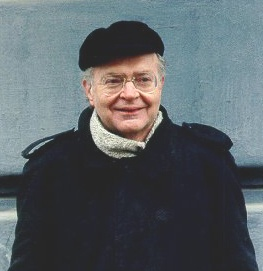
\includegraphics[width=0.6\linewidth]{images/knuth}
    \caption{Knuth}
    \label{fig:my_label2}
\end{figure}


\paragraph*{Актуальность.}

\paragraph*{Цель исследования.}
\paragraph*{Научные задачи.}

\paragraph*{Методы исследования.}


\paragraph*{Основные положения, выносимые на защиту.}
\begin{enumerate}
    \item \statementOneRU
    \item \statementTwoRU 
\end{enumerate}

\paragraph*{Научная новизна.}

\paragraph*{Теоретическая значимость.}
\paragraph*{Практическая значимость.}
\paragraph*{Достоверность.}
\paragraph*{Аппробация работы.}
\paragraph*{Личный вклад автора.}


\paragraph*{Объём и структура работы.}
Диссертация состоит из~введения,
\formbytotal{totalchapter}{глав}{ы}{}{},
заключения и
\formbytotal{totalappendix}{приложен}{ия}{ий}{}.
%% на случай ошибок оставляю исходный кусок на месте, закомментированным
%Полный объём диссертации составляет  \ref*{TotPages}~страницу
%с~\totalfigures{}~рисунками и~\totaltables{}~таблицами. Список литературы
%содержит \total{citenum}~наименований.
%
Полный объём диссертации составляет
\formbytotal{TotPages}{страниц}{у}{ы}{}, включая
\formbytotal{totalcount@figure}{рисун}{ок}{ка}{ков} и
\formbytotal{totalcount@table}{таблиц}{у}{ы}{}.
Список литературы содержит
\formbytotal{citenum}{наименован}{ие}{ия}{ий}.




\newpage
\section*{Основное содержание работы}

В Главе~\ref{ch:ch1}...

\section*{Публикации автора по теме диссертации}


Основные результаты по теме диссертации изложены в \theAllMyPapers~публикациях. 
Из них
%4 изданы в журналах, рекомендованных ВАК, 
\theScopusPapers~опубликовано в изданиях, индексируемых в базе цитирования Scopus. 
%Также имеется 1 свидетельство о государственной регистрации программ для ЭВМ.

В международных изданиях, индексируемых в базе данных Scopus:
\begin{refsection}[biblio/own.bib]
\nocite{*}
\printbibliography[
    keyword=scopus,
    %title={В международных изданиях, индексируемых в базе данных Scopus}, 
    %heading=subbibliography,
    heading=none,
    resetnumbers=true
]
\end{refsection}



В международных изданиях, индексируемых в базе данных Web of Science:
\begin{refsection}[biblio/own.bib]
\nocite{*}
\printbibliography[
    keyword=wos,
    %title={В международных изданиях, индексируемых в базе данных Web of Science}, 
    %heading=subbibliography,
    heading=none,
    resetnumbers=true
]
\end{refsection}
Список всех публикаций автора по теме диссертации:
\begin{refsection}[biblio/own.bib]
\nocite{*}
\printbibliography[
    keyword=own,
    %title={Список всех публикаций автора по теме диссертации}, 
    %heading=subbibliography,
    heading=none,
    resetnumbers=true
]
\end{refsection}
 % реферат на русском

%\renewcommand{\figurename}{Figure}
%\renewcommand{\tablename}{Table}
%\chapter*{Synopsis}
\addcontentsline{toc}{chapter}{Synopsis} 

\begin{center}
    General thesis summary
\end{center}


\paragraph*{Relevance of the chosen topic.}
\paragraph*{Goal.}
\paragraph*{Objectives.}
\paragraph*{Research methods.}
\paragraph*{Assertions that are presented for defense.}
\paragraph*{The novelty of research.}
\paragraph*{The scientific and technical objective.}
\paragraph*{The research object.}
\paragraph*{The research subject.}
\paragraph*{The theoretical significance.}
\paragraph*{The practical significance.}
\paragraph*{The accuracy of the obtained results.}

\paragraph*{Implementation of research results.}
\paragraph*{Approbation of research results.}
\paragraph*{Personal contribution of the author.}
\paragraph*{Thesis structure and number of pages.}

Thesis consists of the introduction,
\formbytotal{totalchapter}{chapter}{}{s}{},
conclusion and 
\formbytotal{totalappendix}{appendix}{}{es}{}.
Thesis is 
\formbytotal{TotPages}{page}{}{s}{} long, including
\formbytotal{totalcount@figure}{figure}{}{s}{} and
\formbytotal{totalcount@table}{table}{}{s}{}.
Bibliography consists of
\formbytotal{citenum}{item}{}{s}{}.


\newpage
\section*{Main contents of the work}

In Chapter~\ref{ch:ch1}...

\section*{Publications.}

Key results of research are described in \theAllMyPapers~publications. 
Among them
%Four of them are published in journals recommended by the Higher Attestation Commission,
\theScopusPapers~is published in a journal indexed by Scopus. 
%One certificate of state registration of a computer program has also been obtained.



Publications in international journals indexed by Scopus:
\begin{refsection}[biblio/own.bib]
\nocite{*}
\printbibliography[
    keyword=scopus,
    %title={В международных изданиях, индексируемых в базе данных Scopus}, 
    %heading=subbibliography,
    heading=none,
    resetnumbers=true
]
\end{refsection}


List of all relevant author's publications:
\begin{refsection}[biblio/own.bib]
\nocite{*}
\printbibliography[
    keyword=own,
    %title={Список всех публикаций автора по теме диссертации}, 
    %heading=subbibliography,
    heading=none,
    resetnumbers=true
]
\end{refsection} % реферат на английском


\renewcommand{\figurename}{Рисунок}
\renewcommand{\tablename}{Таблица}


\chapter*{Введение}                         % Заголовок
\addcontentsline{toc}{chapter}{Введение}    % Добавляем его в оглавление

\paragraph*{Актуальность темы.}

\textbf{Сырая природный газ, добытый из нефтяных скважин, должен быть подвергнут обработке и переработке на газовом заводе, чтобы соответствовать стандартам качества, установленным газопроводными компаниями. Однако, когда питающий газ содержит значительное количество газовых конденсатов (NGL), возникают экономические стимулы для их извлечения, которые обычно могут приносить большую стоимость, чем природный газ с тем же теплотворным эффектом. На рисунке 1 приведена блок-схема газоперерабатывающего завода, предназначенного для производства NGL. Извлеченный поток NGL обычно направляется на фракционирование для дальнейшей переработки в отдельные продукты. Компонент этана может быть продан в качестве сырья для нефтехимических заводов. Пропановые и бутановые жидкости оцениваются как жидкое топливо. Сжиженный газ (LPG), состоящий из пропана и бутана, широко используется как альтернативное топливо для домашних нужд, а также как сырье для химической промышленности. Природный бензин (конденсат C5+) может быть экспортирован в нефтеперерабатывающие заводы в качестве компонента для смешивания с моторным бензином. Гидроуглеводные жидкие продукты из установки фракционирования NGL иногда не соответствуют спецификациям заказчика (см. Таблицу 1). Фактически, если в питательном газе присутствуют кислотные и содержащие серу соединения и они не были удалены до извлечения NGL, они окажутся в продуктах NGL (см. Таблицу 2). Эти жидкие продукты могут потребовать дополнительной обработки для удаления этих загрязнителей. Однако, если эти загрязнители в значительной степени удаляются на этапе подготовки сырья, дальнейшая обработка может быть сокращена или исключена. Существуют две основные причины удаления кислотных газов и соединений серы из углеводородных жидкостей: (1) защита окружающей среды путем уменьшения или исключения количества токсичного сероводорода (H2S) и/или диоксида серы (SO2), высвобождающегося или образующегося во время сгорания, и (2) защита оборудования процесса, контактирующего с кислыми потоками углеводородных жидкостей. Фактически, эти загрязнители могут вызывать коррозию оборудования, если жидкость недостаточно обезвожена. Сероводород достаточно коррозионно активен при концентрациях более 0,55 ppmw, что может привести к провалу испытания на медную полосу для LPG, в то время как 2 ppmw элементарной серы могут вызвать провал испытания на медную полосу (Pyburn et al., 1978). Если присутствуют как сероводород, так и элементарная сера, пороговые значения для провала испытания на медную полосу значительно снижаются (там же). Меркаптаны (RSH) нежелательны в углеводородных жидких продуктах прежде всего из-за запаха. До 100 ppm меркаптанов не приведут к провалу испытания на медную полосу и даже могут обеспечить некоторое торможение реакции H2S с медной полосой (там же). Однако, если также присутствует элементарная сера, меркаптаны вызовут провал испытания на медную полосу.Карбонилсульфид (COS) и дисульфид углерода (CS2), хотя и не коррозионно активны в LPG, медленно гидролизуются до H2S в присутствии свободной воды, что приводит к выходу продукции из спецификации (Nielsen et al., 1997). Если COS не удаляется из потока сырья, он концентрируется в потоке пропана фракционатора. Затем COS может быть обработан с помощью твердых адсорбентов, либо регенерируемых, либо нерегенерируемых (Amiridis, 2006). Наконец, присутствие значительного количества диоксида углерода (CO2) может увеличить паровое давление и снизить теплотворную способность углеводородных жидкостей (Mokhatab et al., 2015). Обратите внимание, что стабилизированный конденсат должен быть подвергнут обработке для удаления тяжелых меркаптанов и других нежелательных загрязнителей до очень низких уровней, чтобы получить жидкий продукт, который соответствует спецификациям для продажи как "природный бензин". В то время как паровая перегонка в стабилизаторе может быть использована для удаления легких углеводородных и кислых газовых компонентов, она имеет минимальное воздействие на удаление тяжелых меркаптанов (Mokhatab et al., 2015). Если конденсат содержит меркаптаны более низкой молекулярной массы (например, метилмеркаптан), его можно обработать с помощью традиционных технологий жидкостной обработки, таких как щелочная промывка, процесс Merox™ от UOP, процесс THIOLEX™ от Merichem, молекулярные сита или твердые катализаторные слои. Если конденсат содержит меркаптаны более высокой молекулярной массы, ароматические сернистые соединения (например, тиофен) и другие нежелательные серные компоненты, его необходимо обрабатывать с помощью гидроочистки, которая является распространенным процессом в нефтеперерабатывающих заводах для десульфурации сырья с высоким содержанием серы (Mokhatab et al., 2015).}

\paragraph*{Цель работы.}

\paragraph*{Задачи работы.}

\paragraph*{Научная новизна работы.}

\paragraph*{Теоретическая и практическая значимость работы.}

\paragraph*{Положения выносимые на защиту.}
\begin{enumerate}
    \item \statementOneRU
    \item \statementTwoRU 
\end{enumerate}

\paragraph*{Апробация работы.}

\paragraph*{Достоверность научных достижений.}

\paragraph*{Внедрение результатов работы.}

\paragraph*{Публикации.} Список всех публикаций автора по теме диссертации:
\begin{refsection}[biblio/own.bib]
\nocite{*}
\printbibliography[
    keyword=own,
    heading=none,
    resetnumbers=true
]
\end{refsection}



\paragraph*{Структура и объем диссертации. }
Диссертация состоит из~введения,
\formbytotal{totalchapter}{глав}{ы}{}{},
заключения и
\formbytotal{totalappendix}{приложен}{ия}{ий}{}.
Полный объём диссертации составляет
\formbytotal{TotPages}{страниц}{у}{ы}{}, включая
\formbytotal{totalcount@figure}{рисун}{ок}{ка}{ков} и
\formbytotal{totalcount@table}{таблиц}{у}{ы}{}.
Список литературы содержит
\formbytotal{citenum}{наименован}{ие}{ия}{ий}.    % Введение


\ifnumequal{\value{contnumfig}}{1}{\counterwithout{figure}{chapter}
}{\counterwithin{figure}{chapter}}
\ifnumequal{\value{contnumtab}}{1}{\counterwithout{table}{chapter}
}{\counterwithin{table}{chapter}}

\chapter{Литературный обзор} \label{ch:ch1}

%------------------------------------------------------------------------------------------
\section{Удаление меркаптанов} \label{sec:ch1/sec1}

Меркаптаны, или, согласно более точному термину, тиолы, представляют собой класс органических соединений, содержащих группу $SH$. Их структурная формула обычно записывается как $RSH$, где $R$ может представлять собой алкильную или ароматическую группу. Меркаптановые компоненты обычно содержаться в природном газе и жидком топливе, таких как бензин, керосин, дизельное топливо. Необходимость удаления меркаптанов обусловлена несколькими факторами:

\begin{enumerate}
	\item Их кислые свойства могут привести к серьезным проблемам с коррозией;
	\item Неприятный запах, обусловленный наличием меркаптанов, требует их удаления из топлива перед сжиганием;
	\item Большинство меркаптанов обладают высокой токсичностью.
\end{enumerate}

Меркаптаны преимущественно представлены низкомолекулярными $C _1$ – $C _3$ прямо-цепными соединениями в составе ПГ и СУГа, в то время как в более тяжелых фракциях присутствуют разветвленные и более высокомолекулярные меркаптаны. Исследования по обработке топлива, содержащего меркаптаны, начались в 1860 году, и традиционные методы удаления основаны на использовании неорганических солей, первый метод «метод докторской очистки» описан в патенте \cite{kalinowski_doctor_1959}. и второй метод так называемая «медная очистка» \cite{krause_color_1952}. В этих методах меркаптаны не удаляются из топлива, а превращаются в дисульфиды, которые не проявляют коррозионную активность и обладают относительно незначительным запахом. Следовательно, содержание серы в топливе не снижается в результате самой очистки обоими упомянутыми традиционными методами.

Метод докторской очистки, который является наиболее старым из них, основан на использовании соли свинца: плумбита натрия ($Na_2PbO_2$). На первом этапе раствор $Na_2PbO_2$, полученный путем растворения оксида свинца в растворе гидроксида натрия ($NaOH$), смешивается с топливом, подлежащим обработке. Меркаптаны в топливе реагируют с $Na_2PbO_2$, образуя свинцовый меркаптид ($(RS)_2Pb$), который растворяется в топливе по реакции \cref{eq:reaction1}:

\begin{equation}
	\mathrm{Na_2PbO_2 + 2RSH \rightarrow {(RS)_2Pb} + 2NaOH} \label{eq:reaction1}
\end{equation}

$(RS)_2Pb$ может быть вновь превращен в $Na_2PbO_2$ с использованием воздуха по реакции \cref{eq:reaction2}: 

\begin{equation}
	\mathrm{(RS)_2Pb + 2NaOH + 1/2O_2 \rightarrow RSSR + Na_2PbO_2 + H_2O} \label{eq:reaction2} 
\end{equation} 

Однако восстановление раствора $Na_2PbO_2$ этим методом происходит медленно и лишь частично. Для полного превращения $(RS)_2Pb$ в дисульфид $(RSSR)$ в реакционную смесь добавляется молекулярная сера, и $(RS)_2Pb$ полностью превращается в свинцовый сульфид $(PbS)$, который выпадает из раствора по реакции \cref{eq:reaction3}:

\begin{equation}
	\mathrm{(RS)_2Pb + S \rightarrow RSSR + PbS} \label{eq:reaction3}
\end{equation} 

Этот процесс обеспечивает полное превращение, однако свинцовый сульфид не может быть восстановлен, поэтому его необходимо утилизировать при завершении реакции. Более того, поскольку сера, добавленная в реакционную смесь для образования дисульфидов, сама растворяется в топливе, содержание серы увеличивается после обработки. В связи с этим данный процесс редко применяется сегодня, за исключением случаев аналитического использования, включенный в стандарты ASTM (ASTM D 4952-09) \cite{noauthor_doctor_nodate}.

Еще один традиционный метод превращения меркаптанов, который называется «медной очисткой» в котором медь используется в виде хлорида ($CuCl_2$). На первом этапе меркаптаны окисляются до дисульфидов по реакции \cref{eq:reaction4}:

\begin{equation}	
	\mathrm{2RSH + 2CuCl_2 \rightarrow RSSR + 2CuCl + 2HCl} \label{eq:reaction4}
\end{equation}

Затем суспензию хлорида меди $(I)$ окисляют снова до хлорида меди $(II)$ с помощью воздуха, в соответствии с реакцией \cref{eq:reaction5}:
\begin{equation}	
	\mathrm{2CuCl + 2HCl + 1/2O_2 \rightarrow 2CuCl_2 + 2H_2O} \label{eq:reaction5}
\end{equation}

Хотя эти процессы все еще используются в некоторых областях, технологии, которые описываются далее, обычно предпочтительнее с точки зрения производительности и затрат.

Существует два основных способа обработки больших объемов меркаптанов в углеводородном сырье: экстракция, где легкие меркаптаны окисляются и удаляются в виде дисульфидов, и очищение, где тяжелые меркаптаны также окисляются, но остаются в потоке. Эти методы применяются при удалении \num{200} кг серы эквивалентов и более в день. Для потоков с меньшим количеством меркаптанов (менее \num{200} кг серы эквивалентов в день) используются альтернативные методы, такие как промывка.

Два основных поставщика лицензий на процессы удаления больших количеств меркаптанов - UOP (Merox\cite{farshi_kinetic_2005}) и GTP-Merichem (Merichem\cite{kohl_gas_1997}). В зависимости от характеристик необходимой степени очистки сырья, каждая компания использует различные конфигурации процессов \cite{bricker_advances_2012, noauthor_mericat_nodate, noauthor_thiolex_nodate}, что отображено в Таблице \cref{tab:remove}.

\begin{table}
	\centering
	\fontsize{12}{15}\selectfont % Установка размера шрифта
	\captionsetup{justification=centering} % выравнивание подписи по-центру
	\caption{Процессы удаления меркаптанов с большим их содержанием \cite{de_angelis_natural_2012}.}\label{tab:remove}
	\begin{tabular}{lllllc}
		\toprule
		Сырье   & Макс. содержание & Процесс      & Процесс    & Содержание после &  \\
		        & до обработки     & Merox        & Merichem   & обработки        &  \\
		        & (ppm Серы)       &              &            &                  &  \\ \midrule
		ПГ      & \num{10000}      & Merox        & Merichem   & Сокращение       &  \\
		СУГ     &                  & Абсорбция,   & Абсорбция, &                  &  \\
		        &                  & Экстракция   & Экстракция &                  &  \\
		Нафта   & \num{5000}       & Экстракция   & Экстракция & Неизменная       &  \\
		бензин  &                  & fixed bed    &            &                  &  \\
		        &                  & sweetening,  &            &                  &  \\
		        &                  & Minalk       &            &                  &  \\
		        &                  & sweetening   &            &                  &  \\
		Нафта   & \num{1000}       & fixed bed    & fixed bed  & Неизменная       &  \\
		Керосин &                  & sweetening,  & sweetening &                  &  \\
		ДТ      &                  & caustic free &            &                  &  \\
		        &                  & sweetening   &            &                  &  \\ \bottomrule
	\end{tabular}
\end{table}

Перед каждым применением процессов Merox или Merichem необходима предварительная щелочная очистка с разведенным раствором гидроксида натрия ($NaOH$), чтобы удалить весь $H_2S$ в сырье. При этом содержание $H_2S$ не должно превышать \num{10} ppm, так как в противном случае $H_2S$ может необратимо реагировать с сильными щелочными растворами, используемыми в процессах Merox или Merichem. Процессы Merox имеют более широкое распространение и масштабы, превышающие \num{1,8} млн. тонн в сутки. К январю \num{2002} года введено в эксплуатацию почти \num{1600} установок с производительностью от \num{5,5} до \num{19,096} тонн в сутки. Для обработки тяжелого сырья, такого как нефть, керосин, дизельное топливо и отопительные масла, также необходима предварительная щелочная очистка для удаления нафтеновых кислот.

Для обработки легкого углеводородного сырья, таких как ПГ или  СУГ, содержащие в себе низкомолекулярные меркаптаны (от метилмеркаптана до бутилмеркаптана), применяются процессы абсорбции и экстракции. На первом этапе газовый поток взаимодействует с концентрированным раствором гидроксида натрия (10-20\% массовой концентрации $NaOH$), в котором меркаптаны растворяются в виде соответствующих натриевых солей по реакции \cref{eq:reaction6}:

\begin{equation}
	\label{eq:reaction6}
	\mathrm{RSH_\text{(газофазная или жидкофазная)} + NaOH \rightarrow RSNa_\text{(жидкофазная)}} 
\end{equation}

На первом этапе процесса, который осуществляется в колонном аппарате, меркаптаны взаимодействуют с щелочным раствором противотоком, в результате чего ПГ или СУГ проходит через верхнюю часть колонны. Вода, содержащая меркаптаны в виде натриевых солей, а также катализатор Merox или Merichem (комплекс фталоцианина кобальта), вытекает из нижней части колонны, затем подогревается и направляется на окисление в регенератор. В регенераторе щелочной раствор реагирует с воздухом, что приводит к окислению меркаптидов до дисульфидов по реакции \cref{eq:reaction7}:

\begin{equation}	
	\mathrm{4RSNa + O_2 + 2H_2O \rightarrow 2RSSR + 4NaOH} \label{eq:reaction7}
\end{equation}

Дисульфиды формируют новую маслянистую фазу, которая тяжелее воды, и эта двухфазная смесь направляется в сепаратор. После этого регенерированный щелочной раствор возвращается в колонну разделения, а маслянистая фаза направляется на соответствующие нужды, например, использование дисульфидного масла как сульфидирущего агента для катализатора гидроочистки, ингибитор коксообразования УЗК и при возможности, продажа как химического реагента. При использовании данных процессов периодически добавляется небольшое количество катализатора для поддержания достаточной эффективности процесса. При обработке методом абсорбции или экстракции меркаптаны превращаются в менее агрессивные и токсичные дисульфиды, а так же и содержание серы в газе уменьшается, поскольку образовавшиеся при окислении меркаптанов дисульфиды удаляются. Прямые операционные расходы оцениваются в \num{4,6} рублей за \num{1} кубический метр очищенного ПГ и \num{230} рублей за \num{1} кубический метр для очистки СУГ.

В таблицах \cref{tab:solid, tab:liquid} приведены наиболее распространенные хемосорбционные процессы для очистки углеводородного сырья в которых содержится малое количество сернистых соединений \cite{foral_evaluation_1995} (обычно менее \num{200} ppm, в пересчете на общую серу) с использованием твердых и жидких поглотителей. Большинство процессов представляют собой стехиометрические реакции между молекулами, содержащими серу, и реагентом, который не может быть восстановлен и должен быть утилизирован. Обычная аминовая очистка (МЕА, ДЕА и МДЕА) не являются экономически выгодными. Эти процессы предназначены для использования, где ежедневное производство соединений серы не превышает \num{185} кг серы в день.  

\begin{table}
	\centering
	\fontsize{12}{15}\selectfont % Установка размера шрифта
	\captionsetup{justification=centering} % выравнивание подписи по-центру
	\caption{Процессы для небольшого количества $H_2S$ и меркаптанов (твердая фаза)\cite{abdulrahman_natural_2012, kohl_gas_1997, de_angelis_natural_2012}.} \label{tab:solid}
	\begin{tabular}{lllllc}
		\toprule
		Название процесса & Активная        & Вид           & Возможность & Максимальная &  \\
		(компания)        & фаза            & процесса      & рецикла     & произв.,     &  \\
		                  &                 &               &             & кг/день      &  \\ \midrule
		Iron sponge       & Оксид железа на & Периодический & нет         & \num{45}     &  \\
		(Connelly-GPM)    & опилках дерева  &               &             &              &  \\
		Sulfatreat        & Гематит         & Периодический & нет         & \num{90}     &  \\
		(Sulfatreat)      &                 &               &             &              &  \\
		Sulphur-Rite      & Оксид железа    & Fixed bed     & нет         & \num{180}    &  \\
		(Merichem)        &                 &               &             &              &  \\
		Low temperature   & Оксид цинка     & Fixed bed     & нет         & \num{135}    &  \\
		zinc oxide (ICI)  &                 &               &             &              &  \\
		Chemsweet         & Оксид цинка +   & Периодический & нет         & \num{18}     &  \\
		(NATCO)           & ацетат цинка    &               &             &              &  \\
		Sulfosorb         & Активный уголь  & Fixed bed     & да          & \num{1,4}    &  \\
		(Calgon           & насыщенный      &               &             &              &  \\
		carbon co.)       & солями меди     &               &             &              &  \\ \bottomrule
	\end{tabular}
\end{table}

\begin{table}
	\centering
	\fontsize{12}{15}\selectfont % Установка размера шрифта
	\captionsetup{justification=centering} % выравнивание подписи по-центру
	\caption{Процессы для небольшого количества $H_2S$ и меркаптанов (жидкая фаза) \cite{de_angelis_natural_2012}.} \label{tab:liquid}
	\begin{tabular}{lllllc}
		\toprule
		Название процесса & Активная            & Вид           & Возможность & Максимальная &  \\
		(компания)        & фаза                & процесса      & рецикла     & произв.,     &  \\
		                  &                     &               &             & кг/день      &  \\ \midrule
		Sulfa-check       & Водный раствор      & Периодический & нет         & \num{90}     &  \\
		(Nalco-Exxon)     & $NaNO_2$            &               &             &              &  \\
		Sulfascrub        & 50\% водный раствор & Периодический & нет         & \num{45}     &  \\
		(Petrolite Co.)   & триазина            &               &             &              &  \\
		The Eliminator    & Раствор триазина    & Периодический & нет         & \num{90}     &  \\
		(Merichem)        &                     &               &             &              &  \\ \bottomrule
	\end{tabular}
\end{table}

%------------------------------------------------------------------------------------------
\subsection{Аппаратурное оформление процесса демеркаптанизации.} \label{sec:ch1/sec2}

Процесс удаления меркаптанов из СУГ может быть реализован различными способами, и выбор конкретного метода зависит от требований качества очистки, объемов обрабатываемого газа, экономической целесообразности и других факторов. На рисунке \cref{fig:ExtPlus} изображена схема экстракции процесса Merox "Extractor Plus" \cite{bricker_advances_2012}.

\begin{figure}
	\centering
	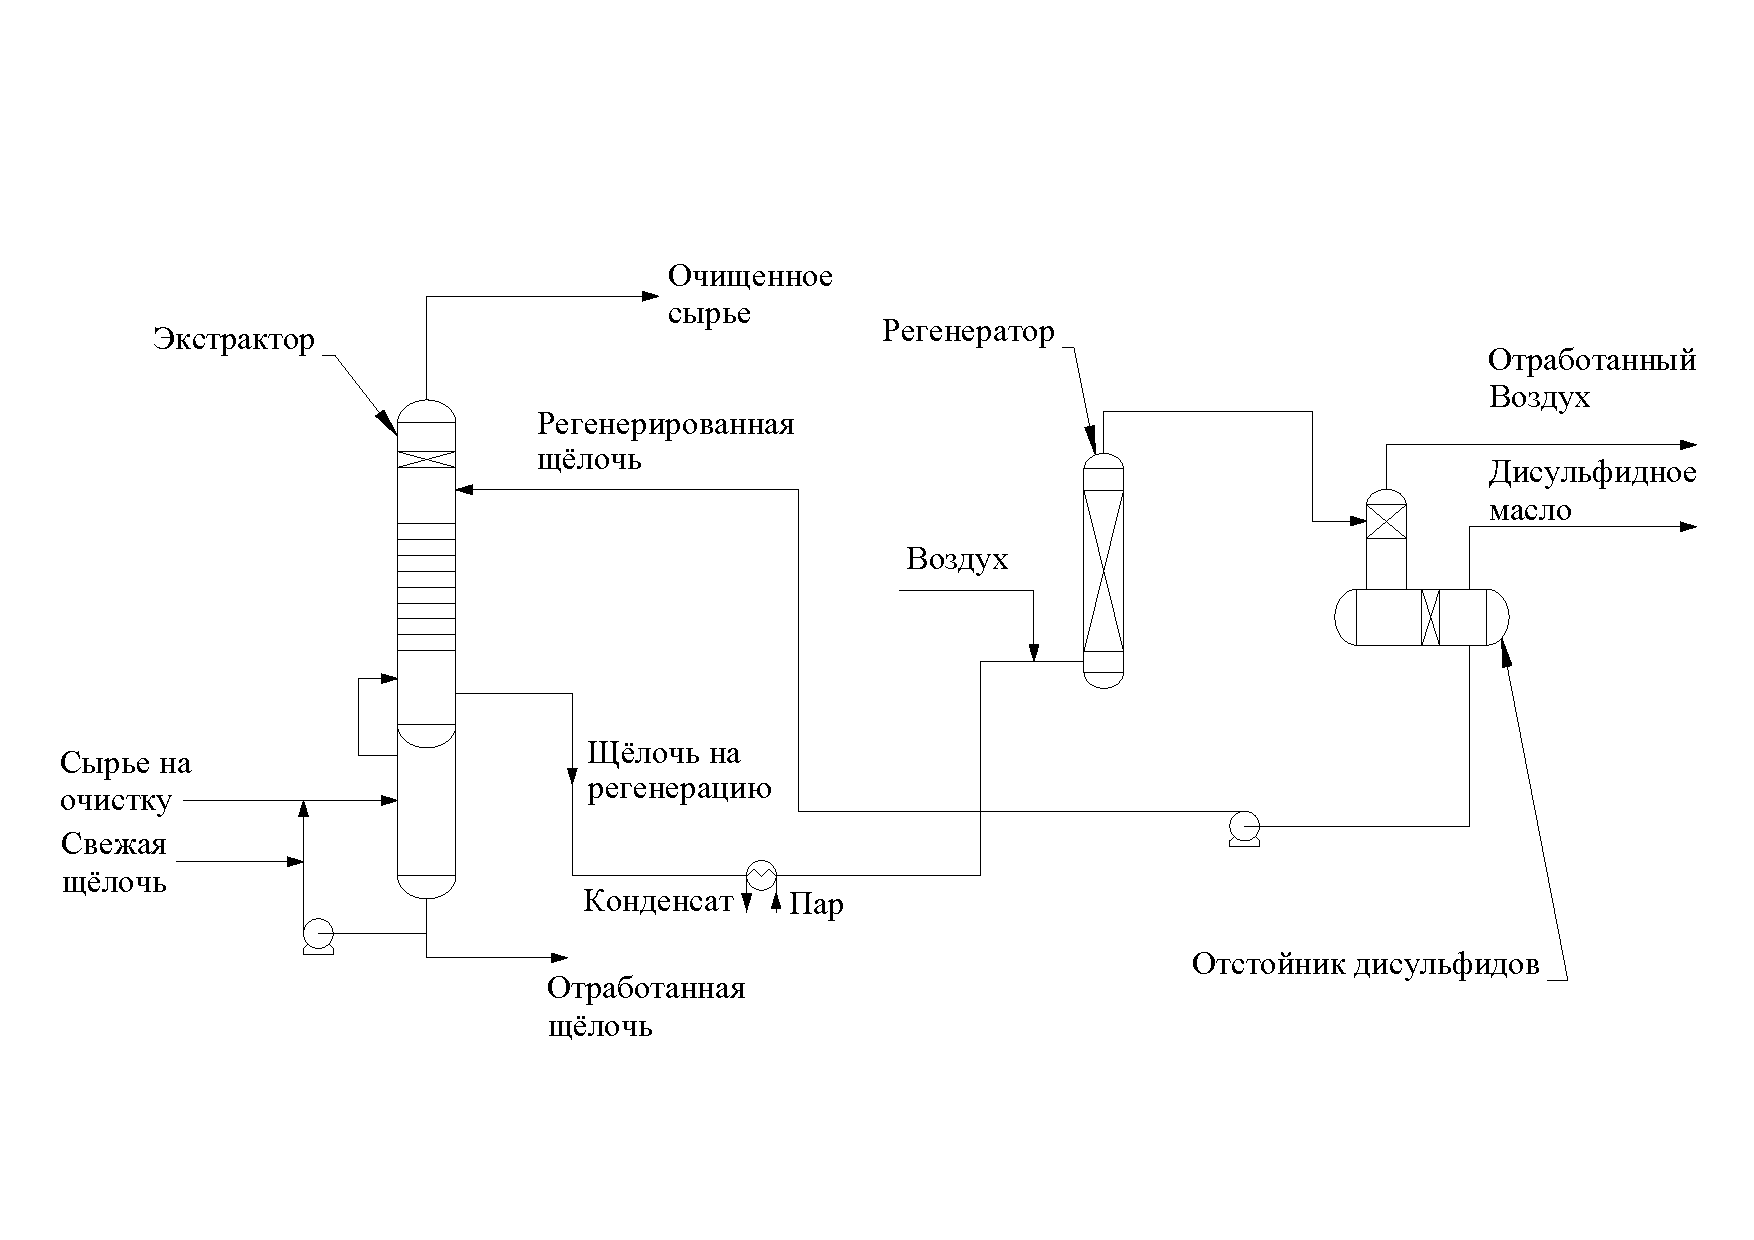
\includegraphics[width=1\linewidth]{images/Extplus}
	\caption{Схема демеркаптанизации компании Merox (Extractor Plus).}
	\label{fig:ExtPlus}
\end{figure}

Это стандартное предложение UOP, где удаление проводят в противоточном тарельчатом либо насадочном экстракторе, данная схема обеспечивает эффективное удаление меркаптановой серы из СУГ. На первом этапе в кубе колонны проводят предварительную очистку сырья с наибольшим содержанием меркаптанов с использованием свежей щелочи для удаления остаточного $H_2S$. Затем, поднимаясь вверх по колонне, сырье которое уже содержит в себе меньше меркаптанов контактирует с регенерированным щелочным раствором. Для обеспечения необходимого уровня удаления меркаптанов рассчитывают необходимый слой насадки или количество тарелок. Противоток в экстракторе обеспечивает благоприятное условие равновесия реакции \cref{eq:reaction6}. В верхней части колонны предусмотрен каплеотбойник для предотвращения уноса щелочи, а из куба колонны насыщенная меркаптидами щелочной раствор поступает на регенерацию. 

Регенерация щелочи осуществляется в отдельной колонне по реакции \cref{eq:reaction7}. Данную окислительную реакцию проводят с избытком воздуха в присутствии катализатора (Merox WSTM), реакция протекает только в сторону образования продукта и более высокая температура до \num{70}°C способствует увеличению скорости реакции. Merox WSTM - это гомогенный катализатор фталоцианина кобальта, который позволяет восстановить щелочной раствор путем окисления меркаптидов до дисульфидов. Отработанный воздух сепарируется из отстойника дисульфидов, а дисульфидное масло отправляется на нужды потребителю, регенерированная щелочь с малым содержанием меркаптидов возвращается в экстрактор.

\begin{figure}
	\centering
	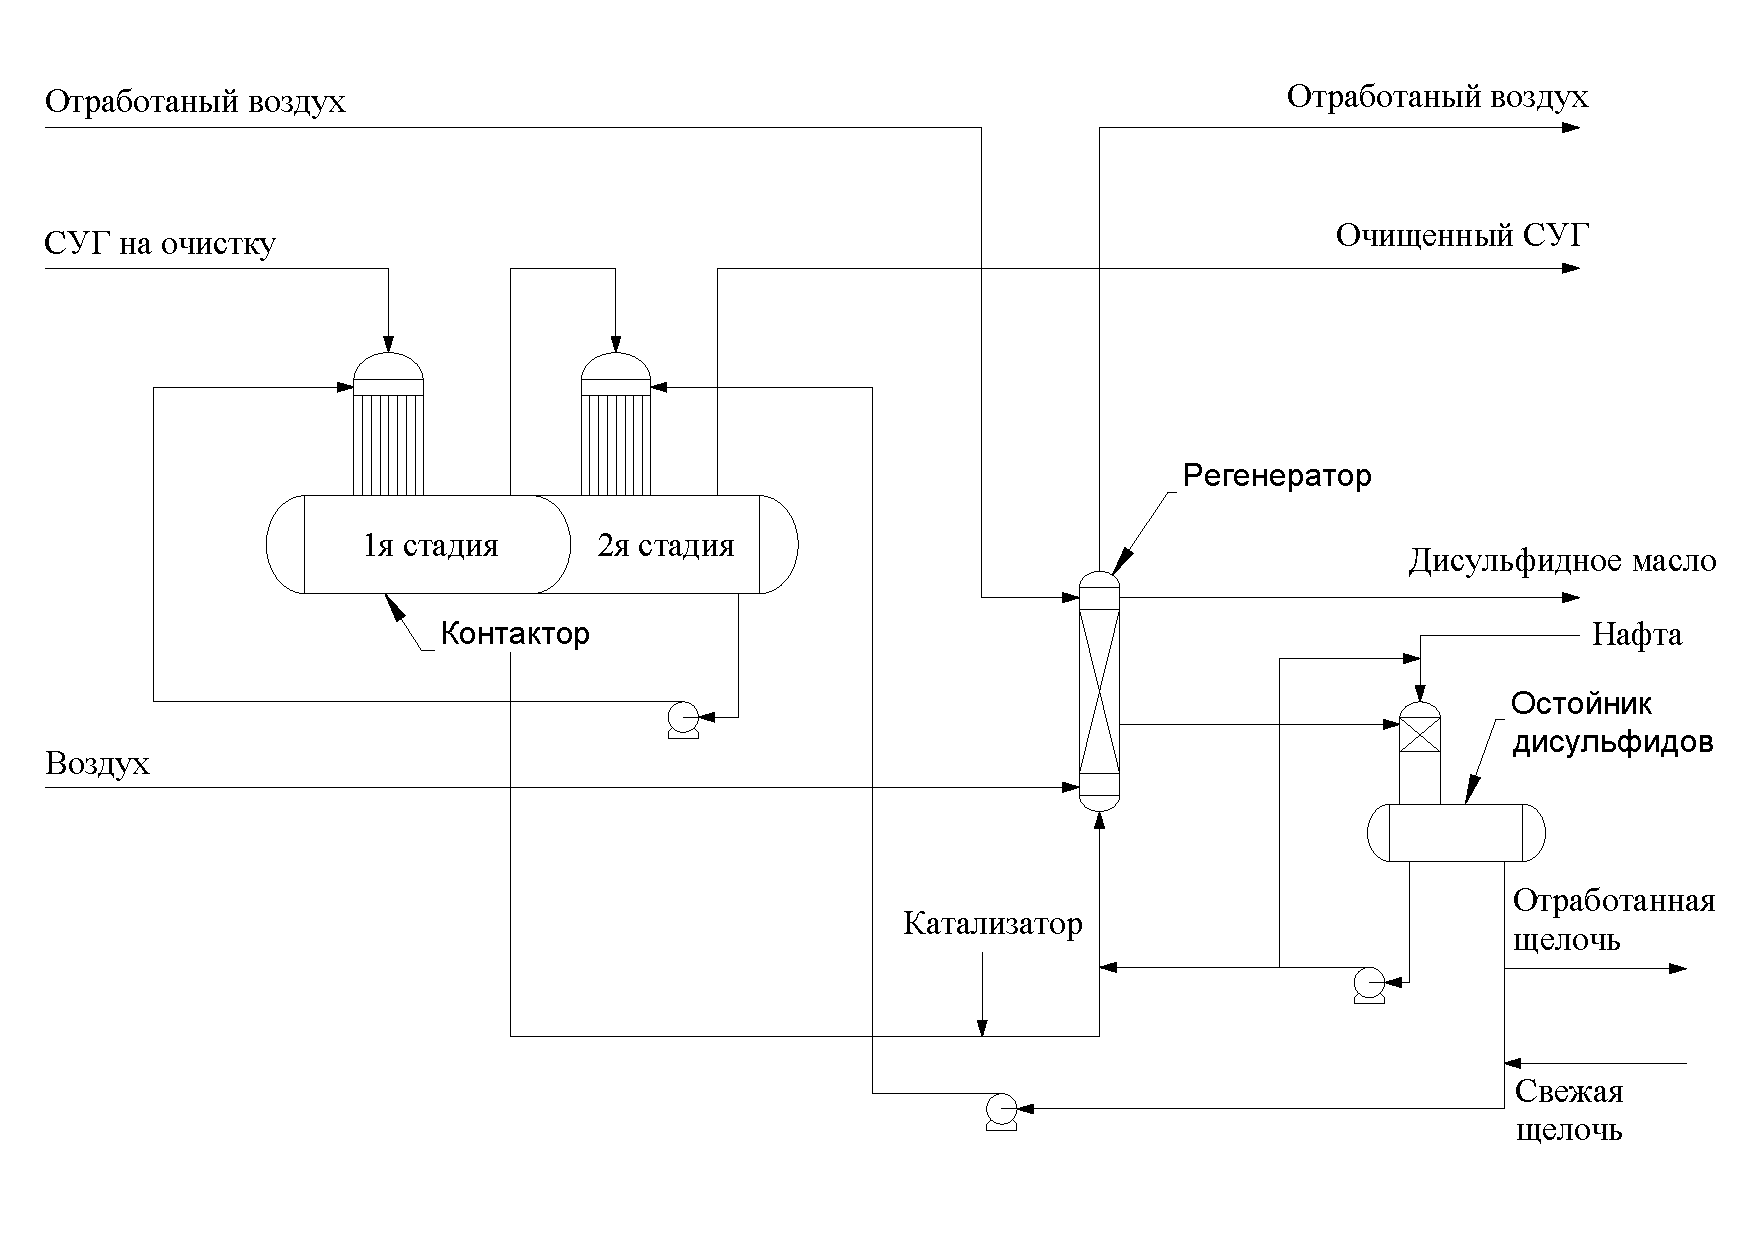
\includegraphics[width=1\linewidth]{images/Eth}
	\caption{Схема двухсекционной демеркаптанизации компании Merichem (THIOLEX).}
	\label{fig:THIOLEX}
\end{figure}

\begin{figure}
	\centering
	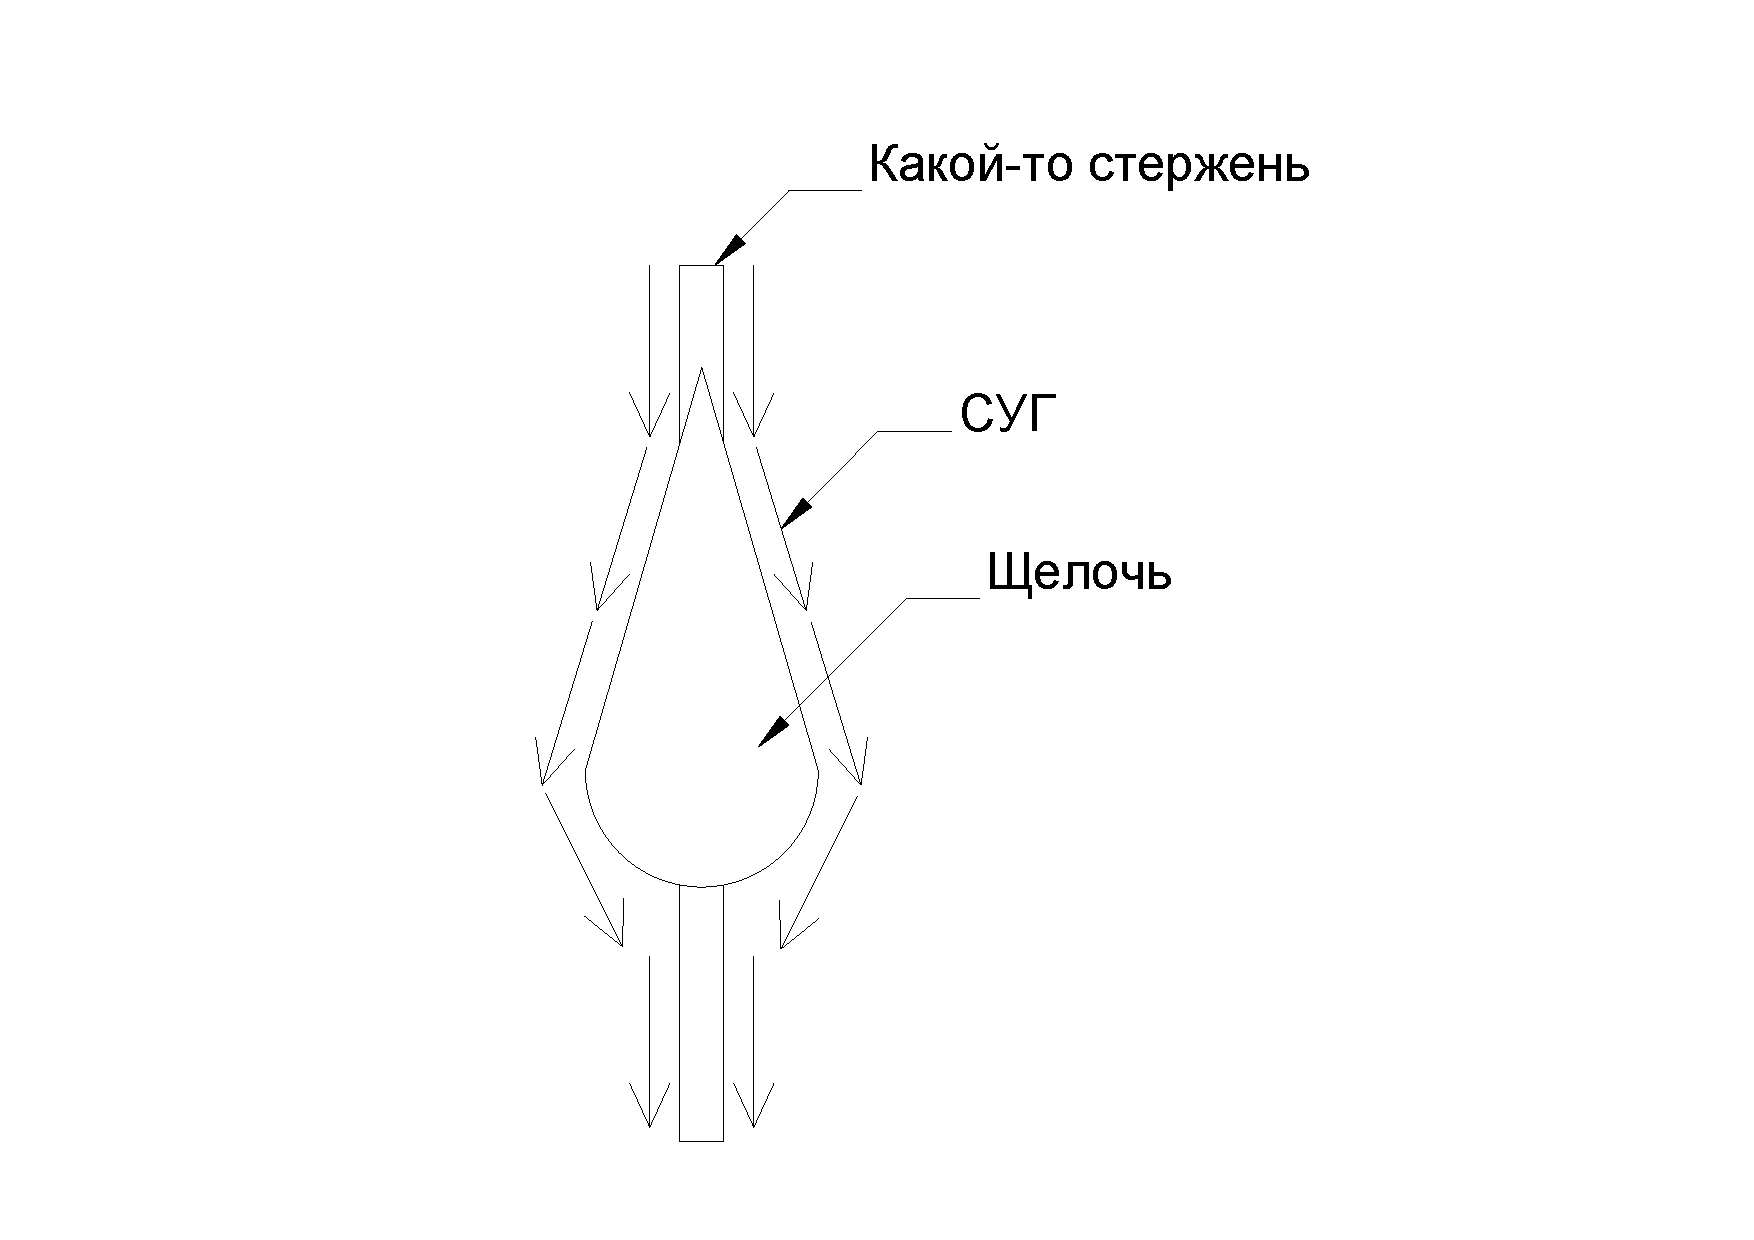
\includegraphics[width=0.6\linewidth]{images/fibr}
	\caption{Схема работы фиброволокнистого контактного устройства компании Merichem.}
	\label{fig:FIBERFILM}
\end{figure}

Так же стоит отметить предложение от компании Merichem рисунок \cref{fig:THIOLEX}, 
процесс THIOLEX, демеркаптанизацию проводят в двухсекционном отстойнике, где щелочная раствор смачивает фиброволокнистое контактное устройство рисунок \cref{fig:FIBERFILM}, затем СУГ стекает по смоченному щелочью контактному устройству и на поверхности раздела фаз реагирует с ней, $H_2S$ и меркаптаны переходят щелочную фазу в виде сульфидов и меркаптидов натрия. Обе фазы отделяются друг от друга в двухсекционном отстойнике, насыщенный сульфидами и меркаптидами натрия щелочной раствор выводится с нижней части отстойника и под собственным давлением направляется на регенерацию, а очищенный до \num{10} ppm c первой секции СУГ поступает на доочистку во вторую секцию отстойника и очищается до \num{5} ppm, так же отмечено что происходит унос щелочного раствора до \num{0,1} ppm. Регенерацию проводят в колонне, где насыщенный щелочной раствор с гомогенным катализатором поднимаясь верх по колонне контактирует с воздухом и происходит окисление содержащихся в щелочном растворе сульфидами и меркаптидами натрия до дисульфидов. Для снижения плотности дисульфидного масла, с целью облегчения его отделения от щелочного раствора в отстойнике дисульфидов, в отстойник подается расчетное количество нафты. Дисульфидное масло с более низким значением плотности, выводится из колонны регенератора для отгрузки на потребительские нужды.

%-----------------------------------------------------------------------------------------------------
\subsection{Влияние контактных устройств на гидродинамику и массообмен процесса.} \label{sec:ch1/sec3}

Схема противоточной системы хемосорбцонной экстракции из двух (частично) растворимых друг в друге жидкостей СУГ и водно-щелочной раствор представлена на рисунке \cref{fig:cheme}.

\begin{figure}
	\centering
	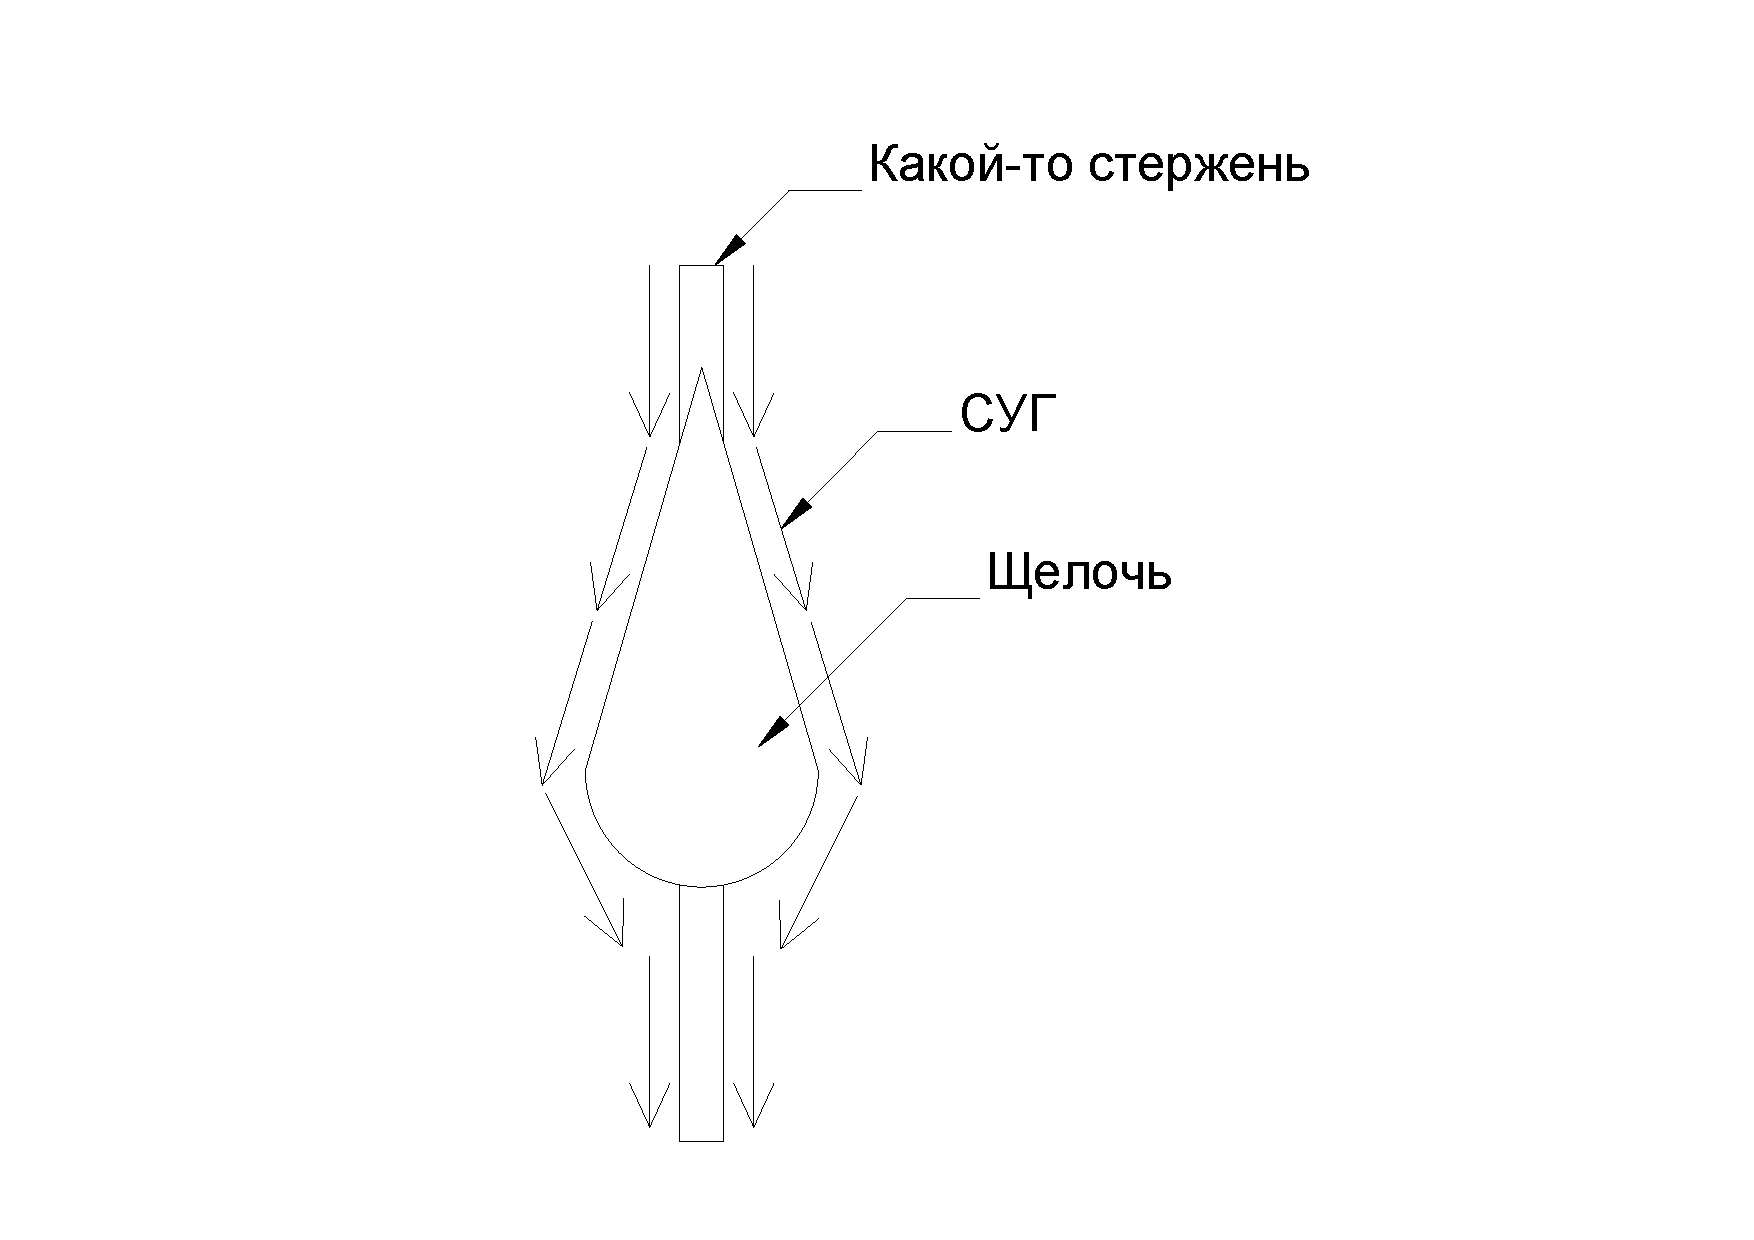
\includegraphics[width=0.6\linewidth]{images/fibr}
	\caption{Заглушка.}
	\label{fig:cheme}
\end{figure}

Взаимодействие фаз в процессе демеркаптанизации может происходить как ступенчато, так и непрерывно. Процесс ступенчатого взаимодействия осуществляется в смесительно-отстойных аппаратах \cref{fig:THIOLEX}, в то время как непрерывное взаимодействие происходит в колонных аппаратах \cref{fig:ExtPlus}. В колоннах противоточное движение фаз осуществляется за счет действия силы тяжести, вызванной разницей плотностей фаз.

Колонные аппараты характеризуются низкой эффективностью из-за ограниченной поверхности контакта фаз, обусловленной большими размерами капель. Кроме того, в аппаратах с размерами более $1,5$ метров наблюдаются значительные поперечные неравномерности (масштабные эффекты), что приводит к снижению эффективности разделения смеси.

Одним из распространенных аппаратов для процесса демеркаптанизации являются колонны с ситчатыми тарелками. В них водно-щелочная фаза заполняет всю колонну и перемещается с тарелки на тарелку, тогда как другая дисперсная фаза (СУГ) диспергируется через отверстия на тарелках, перемещается в пространстве между тарелками и, достигая следующей тарелки, коалесцирует. Этот процесс диспергирования и коалесцирования происходит многократно, увеличивая интенсивность процесса демеркаптанизации. Присутствие ситчатых тарелок способствует уменьшению обратного перемешивания. Также применяются аппараты с насадкой, пульсационные и вибрационные аппараты.

 
\subsection{Диффузионные процессы химической технологии.} \label{sec:ch1/sec4}

Диффузионные процессы, при которых меняется состав обеих фаз, выгодно проводить по принципу

В химической технологии большое значение имеют процессы диффузионного обмена веществом между фазами. Сюда относятся процессы абсорбции (поглощения газов жидкостями) и экстракции (перенос вещества между двумя несмешивающимися жидкими фазами). Поглощение газа жидкостью подобно процессу конденсации, с той лишь разницей, что к диффузионному сопротивлению газа добавляется диффузионное сопротивление конденсированной фазы. Если абсорбция не сопровождается медленными химическими реакциями, то на поверхности устанавливается равновесие между концентрациями диффундирующего вещества в газовой и жидкой фазах. При стационарном протекании процесса он может быть описан моделью двух пленок: газовой и жидкой. Как и всегда в подобных случаях, действует закон сложения последовательным сопротивлений \cref{eq:equation1}:
 
\begin{equation}
	\label{eq:equation1}
	\begin{alignedat}{2}
		j_1 = \frac{xC^0_\text{газ} - C^0_\text{жидкость}}{\frac{1}{\beta_\text{жидкость}} + \frac{x}{\beta_\text{газ}}} = \frac{C^0_\text{газ} - \frac{C^0_\text{жидкость}}{x}}{{\frac{1}{\beta_\text{жидкость}} + \frac{1}{x\beta_\text{ж}}}}
	\end{alignedat}
\end{equation}\\
где x - равновесная растворимость;

Величины, стоящие в знаменателе, представляют собой диффузионные сопротивления газовой и жидкой пленок, отнесенные к концентрациям либо в жидкой, либо в газовой фазе.

Диффузионные процессы, при которых меняется состав обеих фаз, выгодно проводить по принципу противотока: газ и жидкость поступают с противоположных концов аппарата (газ снизу, жидкость сверху). Таким образом используется наибольшая доступная разность концентраций. При расчете противоточных процессов удобно ввести понятие теоретической тарелки пли ступени переноса. При этом непрерывный процесс переноса приближенно заменяется ступенчатым и принимается, что на каждой ступени устанавливается равновесие между фазами. Необходимое число теоретических тарелок находится простым графическим методом: строится диаграмма, в которой по двум осям отложены концентрации рассматриваемого компонента в двух фазах. На этой диаграмме проводятся линия равновесия по закону растворимости и рабочая линия по уравнению материального баланса. Ступенчатый процесс представляется на диаграмме ломаной, прямоугольные ступеньки которой лежат между линией равновесия и рабочей линией. Число теоретических тарелок равно числу ступенек этой линии. 

В тарельчатых колоннах необходимое число действительных тарелок находится умножением числа теоретических тарелок на коэффициент полезного действия тарелки, находимый раз навсегда экспериментальным. В насадочных колоннах (скрубберах) опреде-ляется экспериментально длина насадки, эквивалентная одной теоретической тарелке. В аппаратах с пробулькивапием (барбoтажем) из эксперимента находится высота подъема пузырьков, эквивалентная теоретической тарелке. 

Метод теоретических тарелок позволяет, таким образом, для противоточных аппаратов обойти расчет самого диффузионного процесса: он заменяется расчетом равновесия, дополненным эмпирическими коэффициентами. Если известны коэффициенты переноса, то длину, эквивалентную одной теоретической тарелке, или коэффициент полезного действия можно рассчитать. Для тарельчатых колонн естественным представляется нестационарный метод расчета коэффициента полезного действия, подробно разработанный Кишиневским [8]. В этом методе рассматривается нестационарпый процесс диффузии для жидкой частицы за время ее пребывания на тарелке, без пользования понятием приведенной пленки. Для насадочиых колонн успешно применяется стационарный метод расчета в приближении двойной пленки; при этом число теоретических тарелок выражается через число единиц переноса (ЧЕП), которое, согласно формуле (III, 38а), связано с критерием Стэптопа. Изложение этого вопроса можно найти в монографии Рамма [9], к которой и отсыпаем интересующегося читателя. Анализ, учитывающий процессы не только диффузии, но и теплолередачи, дал Жаворопков [10]. 

           % Глава 1
\chapter{Вторая глава}
\label{ch:ch2}
           % Глава 2
\chapter{Третья глава}
\label{ch:ch3}

           % Глава 3
\chapter{Четвертая глава}
\label{ch:ch4}           % Глава 4

\chapter*{Заключение}                       % Заголовок
\addcontentsline{toc}{chapter}{Заключение}  % Добавляем его в оглавление


      % Заключение
% Если оч надо это автоматизировать, то смотри здесь
% https://www.overleaf.com/learn/latex/Nomenclatures
%\printnomenclature[3.5cm] % Значение ширины столбца с обозначениями стоит подбирать вручную
        % Список сокращений и условных обозначений
\chapter*{Список используемых терминов и сокращений}             % Заголовок
\addcontentsline{toc}{chapter}{Список сокращений}  % Добавляем его в оглавление

\textbf{ПГ} : Природный газ

\textbf{СУГ} : Сжиженный углеводородный газ
      % Словарь терминов
\clearpage
\ifdefmacro{\microtypesetup}{\microtypesetup{protrusion=false}}{} % не рекомендуется применять пакет микротипографики к автоматически генерируемым спискам
\listoffigures  % Список изображений

%%% Список таблиц %%%
% (ГОСТ Р 7.0.11-2011, 5.3.10)
\clearpage
\listoftables   % Список таблиц
\ifdefmacro{\microtypesetup}{\microtypesetup{protrusion=true}}{}
\newpage           % Списки таблиц и изображений (иллюстративный материал)
% https://tex.stackexchange.com/a/202797
\AtNextBibliography{\setcounter{citenum}{0}}
\printbibliography      % Список литературы
\chapter*{Благодарности}
\addcontentsline{toc}{chapter}{Благодарности} % Благодарности

\setcounter{totalchapter}{\value{chapter}} % Подсчёт количества глав

%%% Настройки для приложений
\appendix
% Оформление заголовков приложений ближе к ГОСТ:
\setlength{\midchapskip}{20pt}
\renewcommand*{\afterchapternum}{\par\nobreak\vskip \midchapskip}
\renewcommand\thechapter{\Asbuk{chapter}} % Чтобы приложения русскими буквами нумеровались

\chapter{Что-то очень важное}
\label{app:details}

\[
    \sin(x) \approx x
\]


\chapter{Основные публикации автора по теме диссертации}
\label{app:publications}

% Нужно разкоментить чтобы появлиась публикация
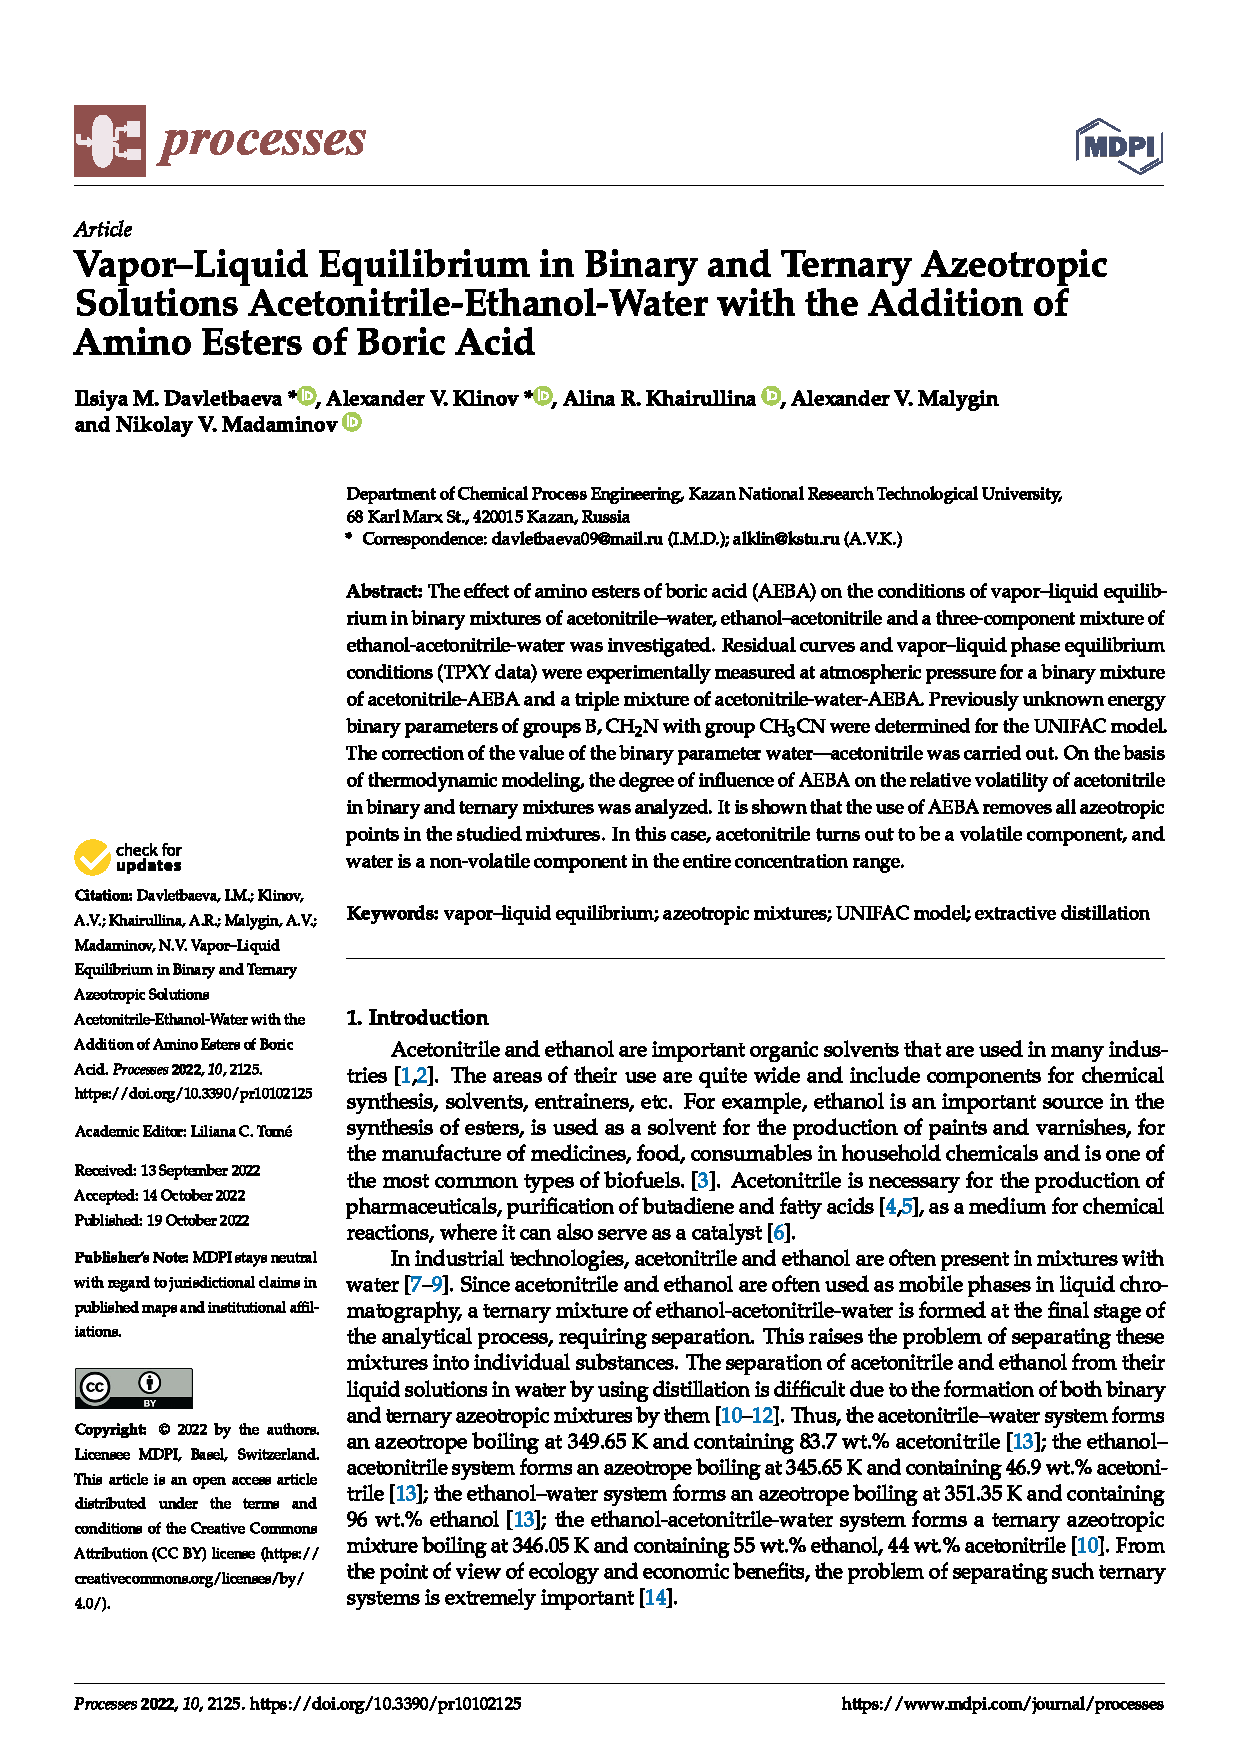
\includepdf[
    pages={-},  % include all pages
    pagecommand={},  % to include global numbering
    scale=0.85,  % to leave space for the global page numbers
    frame,  % adds a frame, optional
]{biblio/MyPublications/processes-10-02125.pdf}

        % Приложения, тут же свои публикации

\setcounter{totalappendix}{\value{chapter}} % Подсчёт количества приложений


\end{document}
